%%%%%%%%%%%%%
%Coverage plots
%Identity figures, uncomment

\begin{figure}[!hbtp]
  \centering
  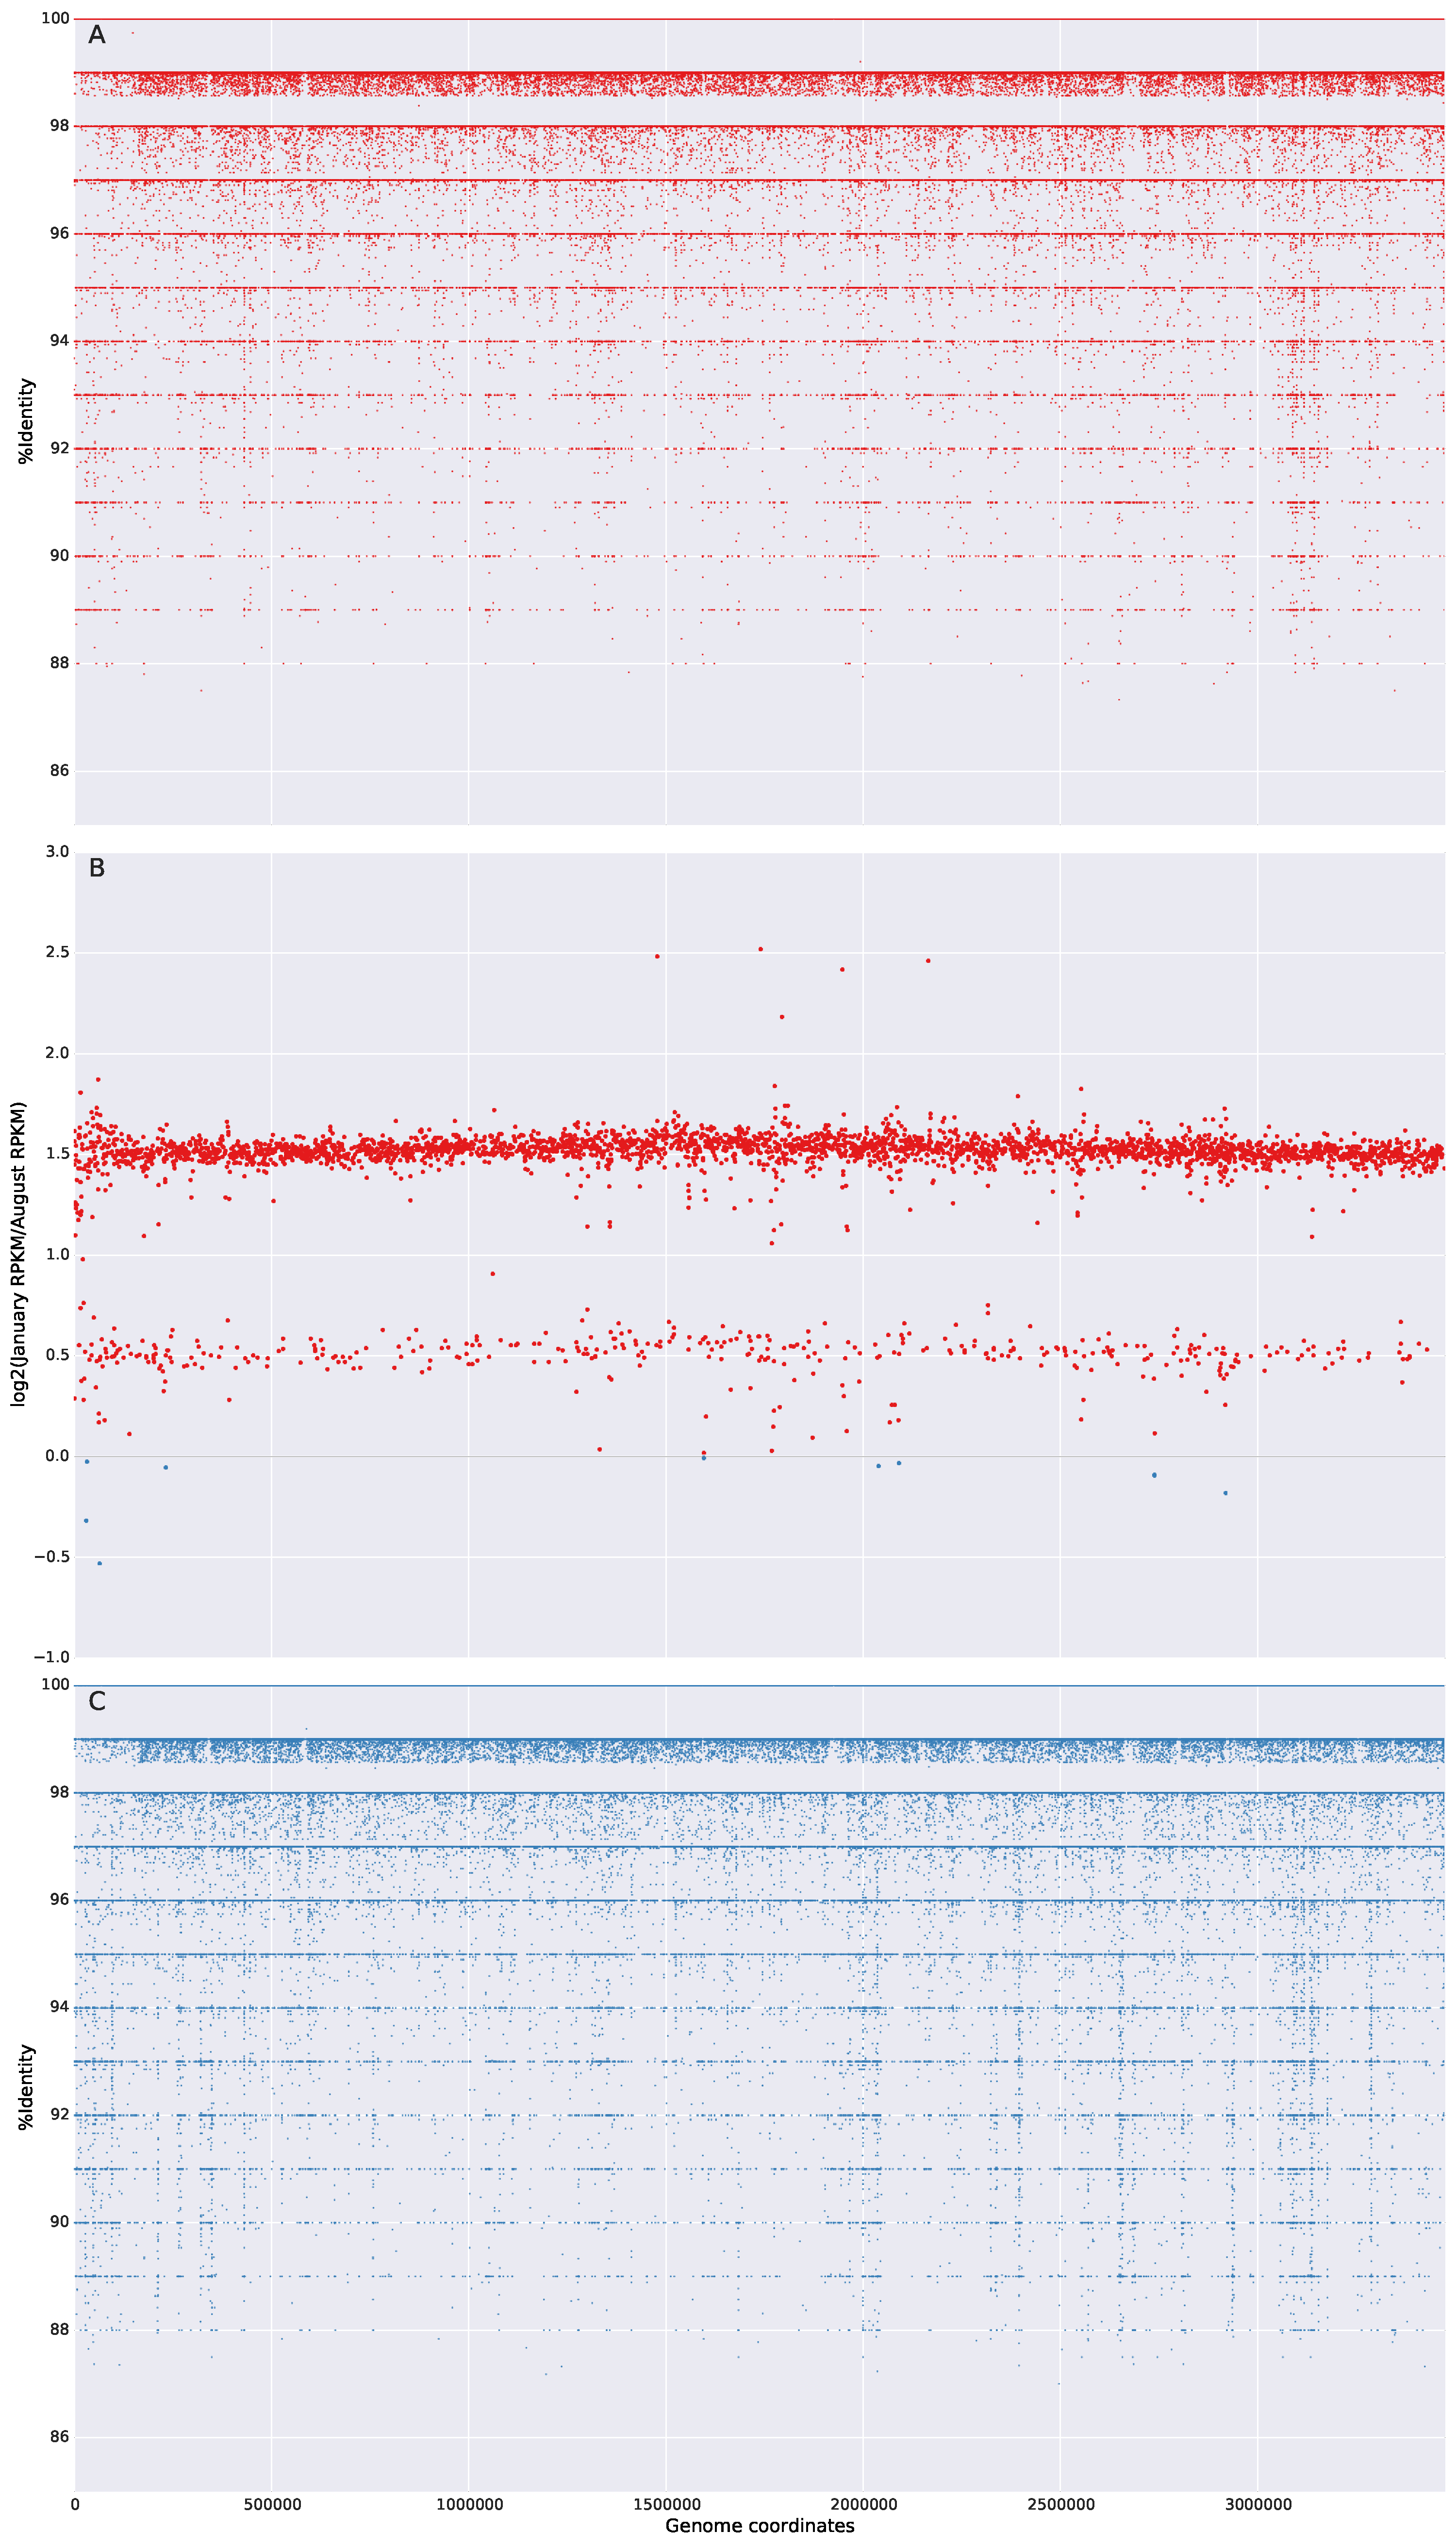
\includegraphics[width=\textwidth,height=0.8\textheight,keepaspectratio]{Chapter5/Figures/coverage_plots/J07HWQ1_coverage.pdf}
  \caption{Coverage and gene abundance for J07HQW1. \textbf{A} and \textbf{C} shows reads recruited to the January and August genomes, respectively. \textbf{B} indicates the number of reads recruited to each individual gene, expressed as RPKM values, where the color indicates the sample from where the read originated (January vs. August.)}
  \label{J07HWQ1coverage}
\end{figure}


\begin{figure}[!hbtp]
  \centering
  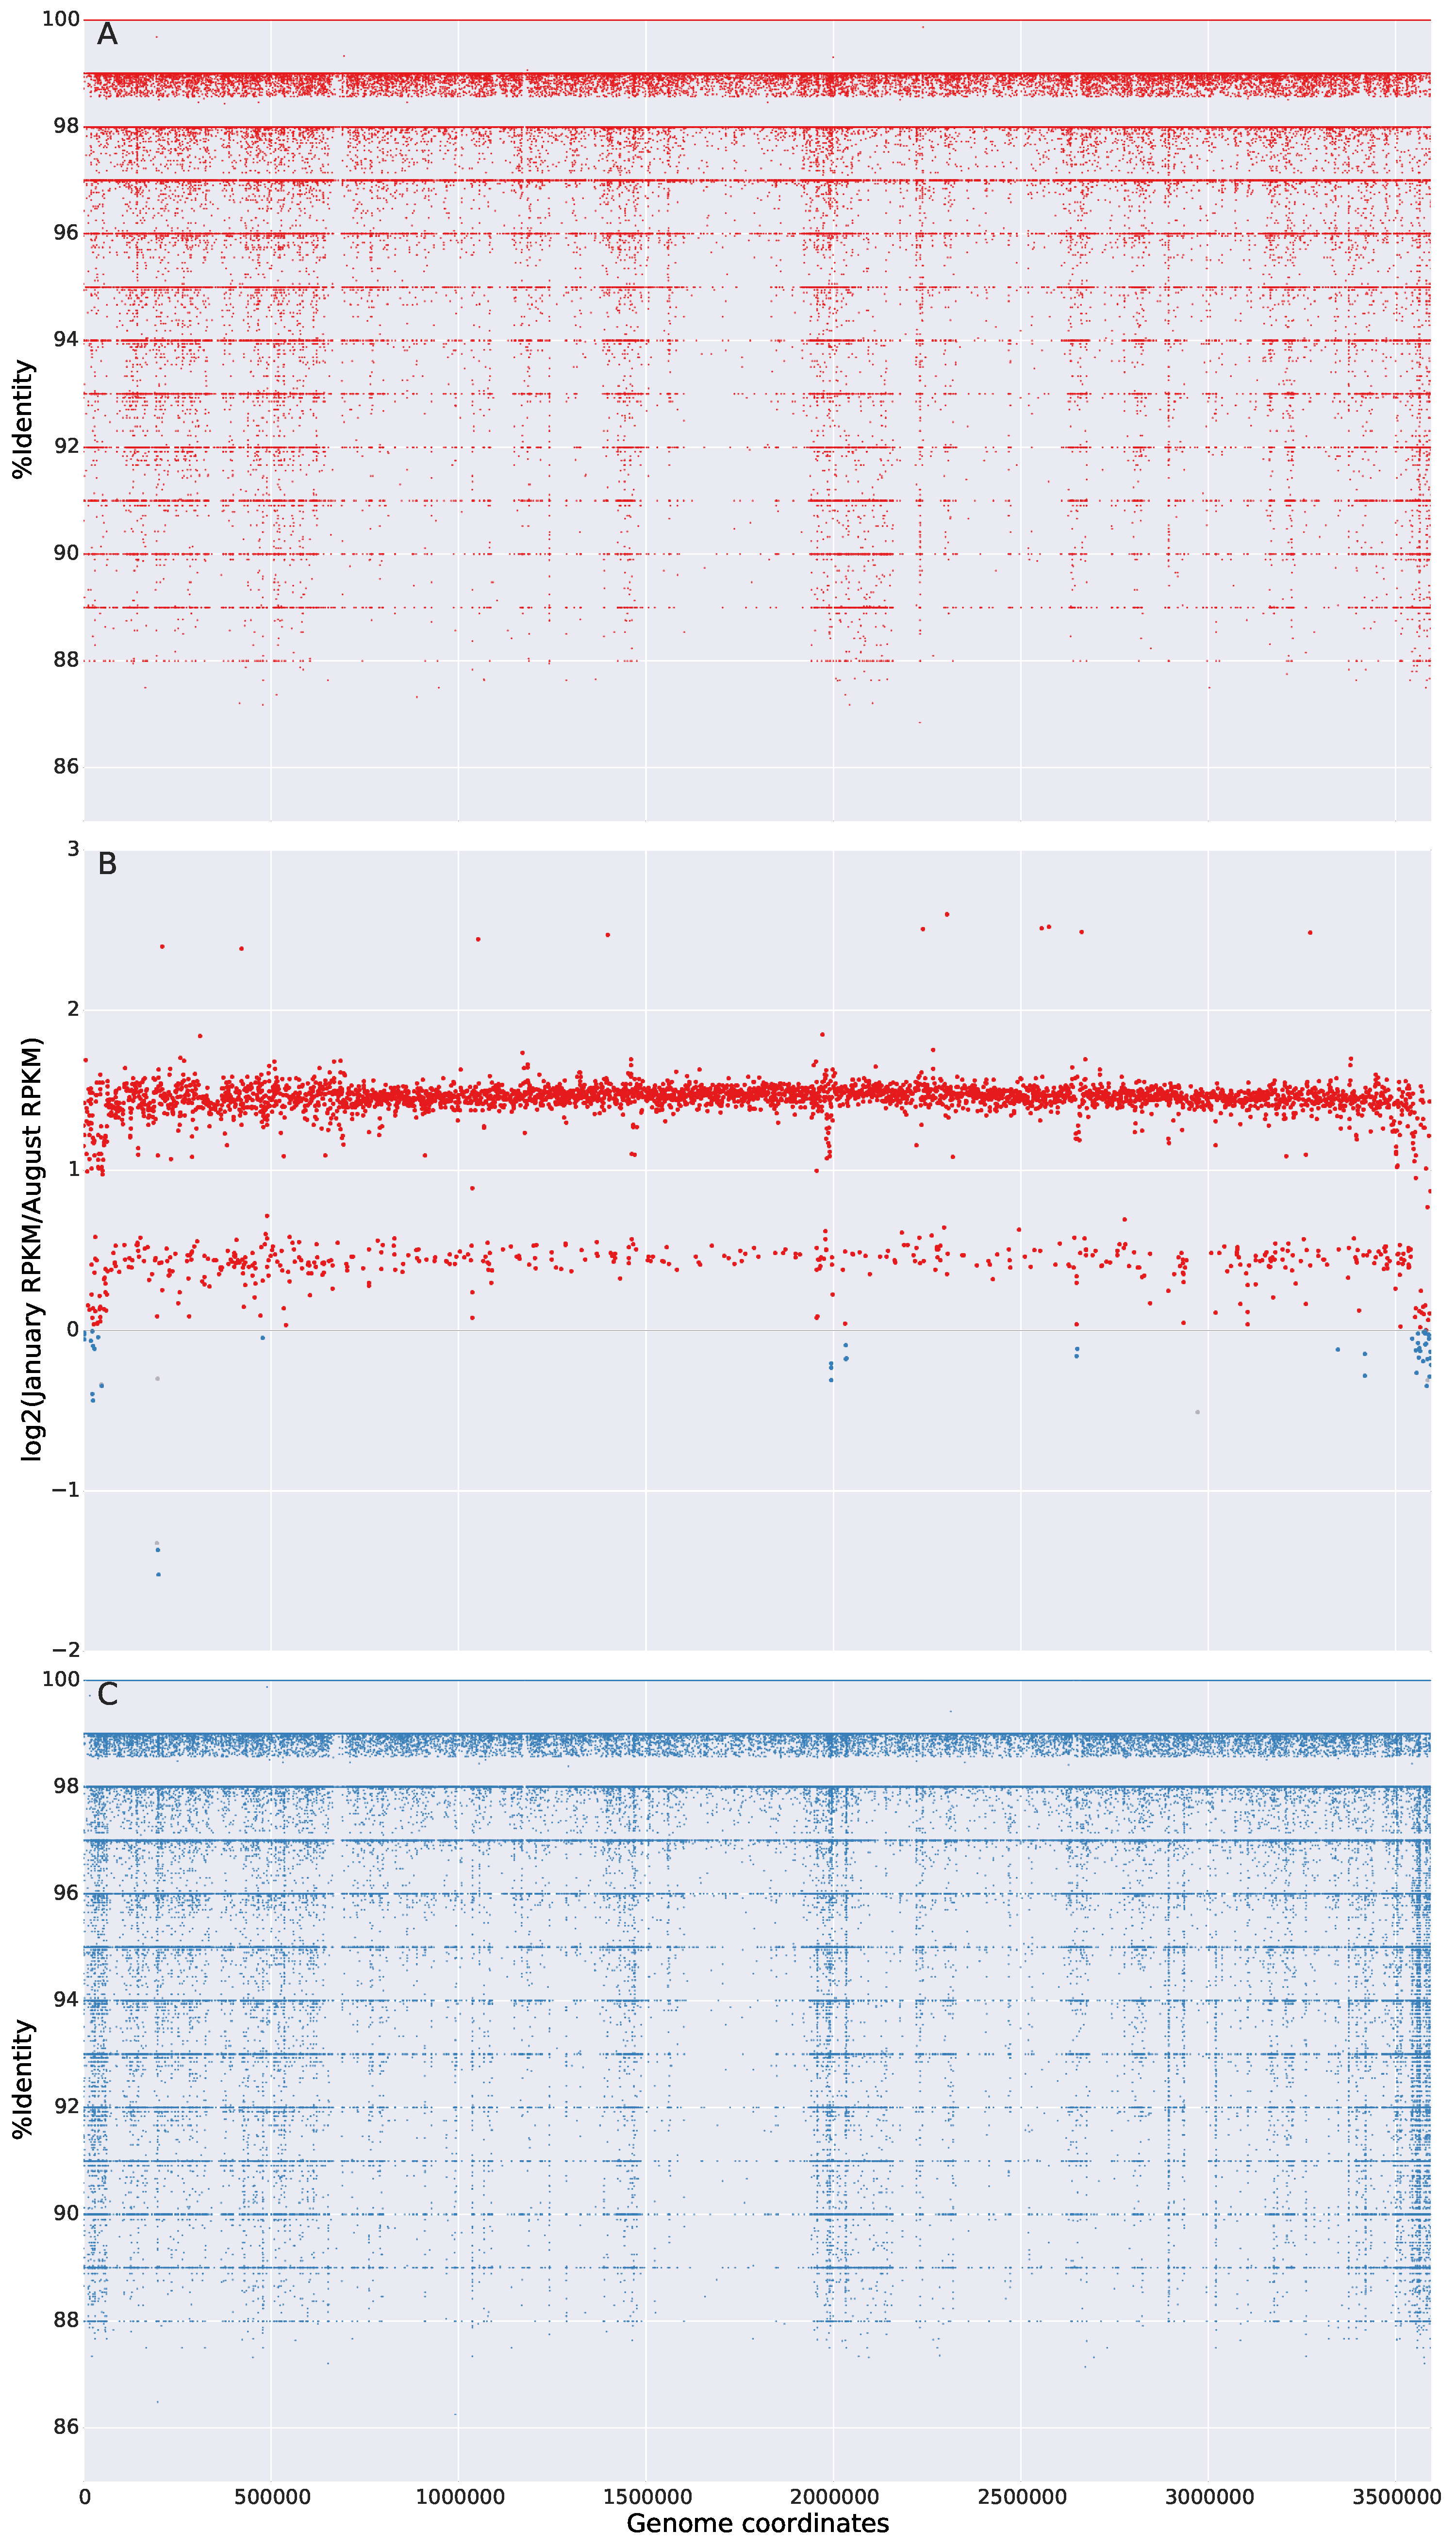
\includegraphics[width=\textwidth,height=0.8\textheight,keepaspectratio]{Chapter5/Figures/coverage_plots/J07HWQ2_coverage.pdf}
  \caption{Coverage and gene abundance for J07HQW2. \textbf{A} and \textbf{C} shows reads recruited to the January and August genomes, respectively. \textbf{B} indicates the number of reads recruited to each individual gene, expressed as RPKM values, where the color indicates the sample from where the read originated (January vs. August.)}
  \label{J07HWQ2coverage}
\end{figure}

\begin{figure}[!hbtp]
  \centering
  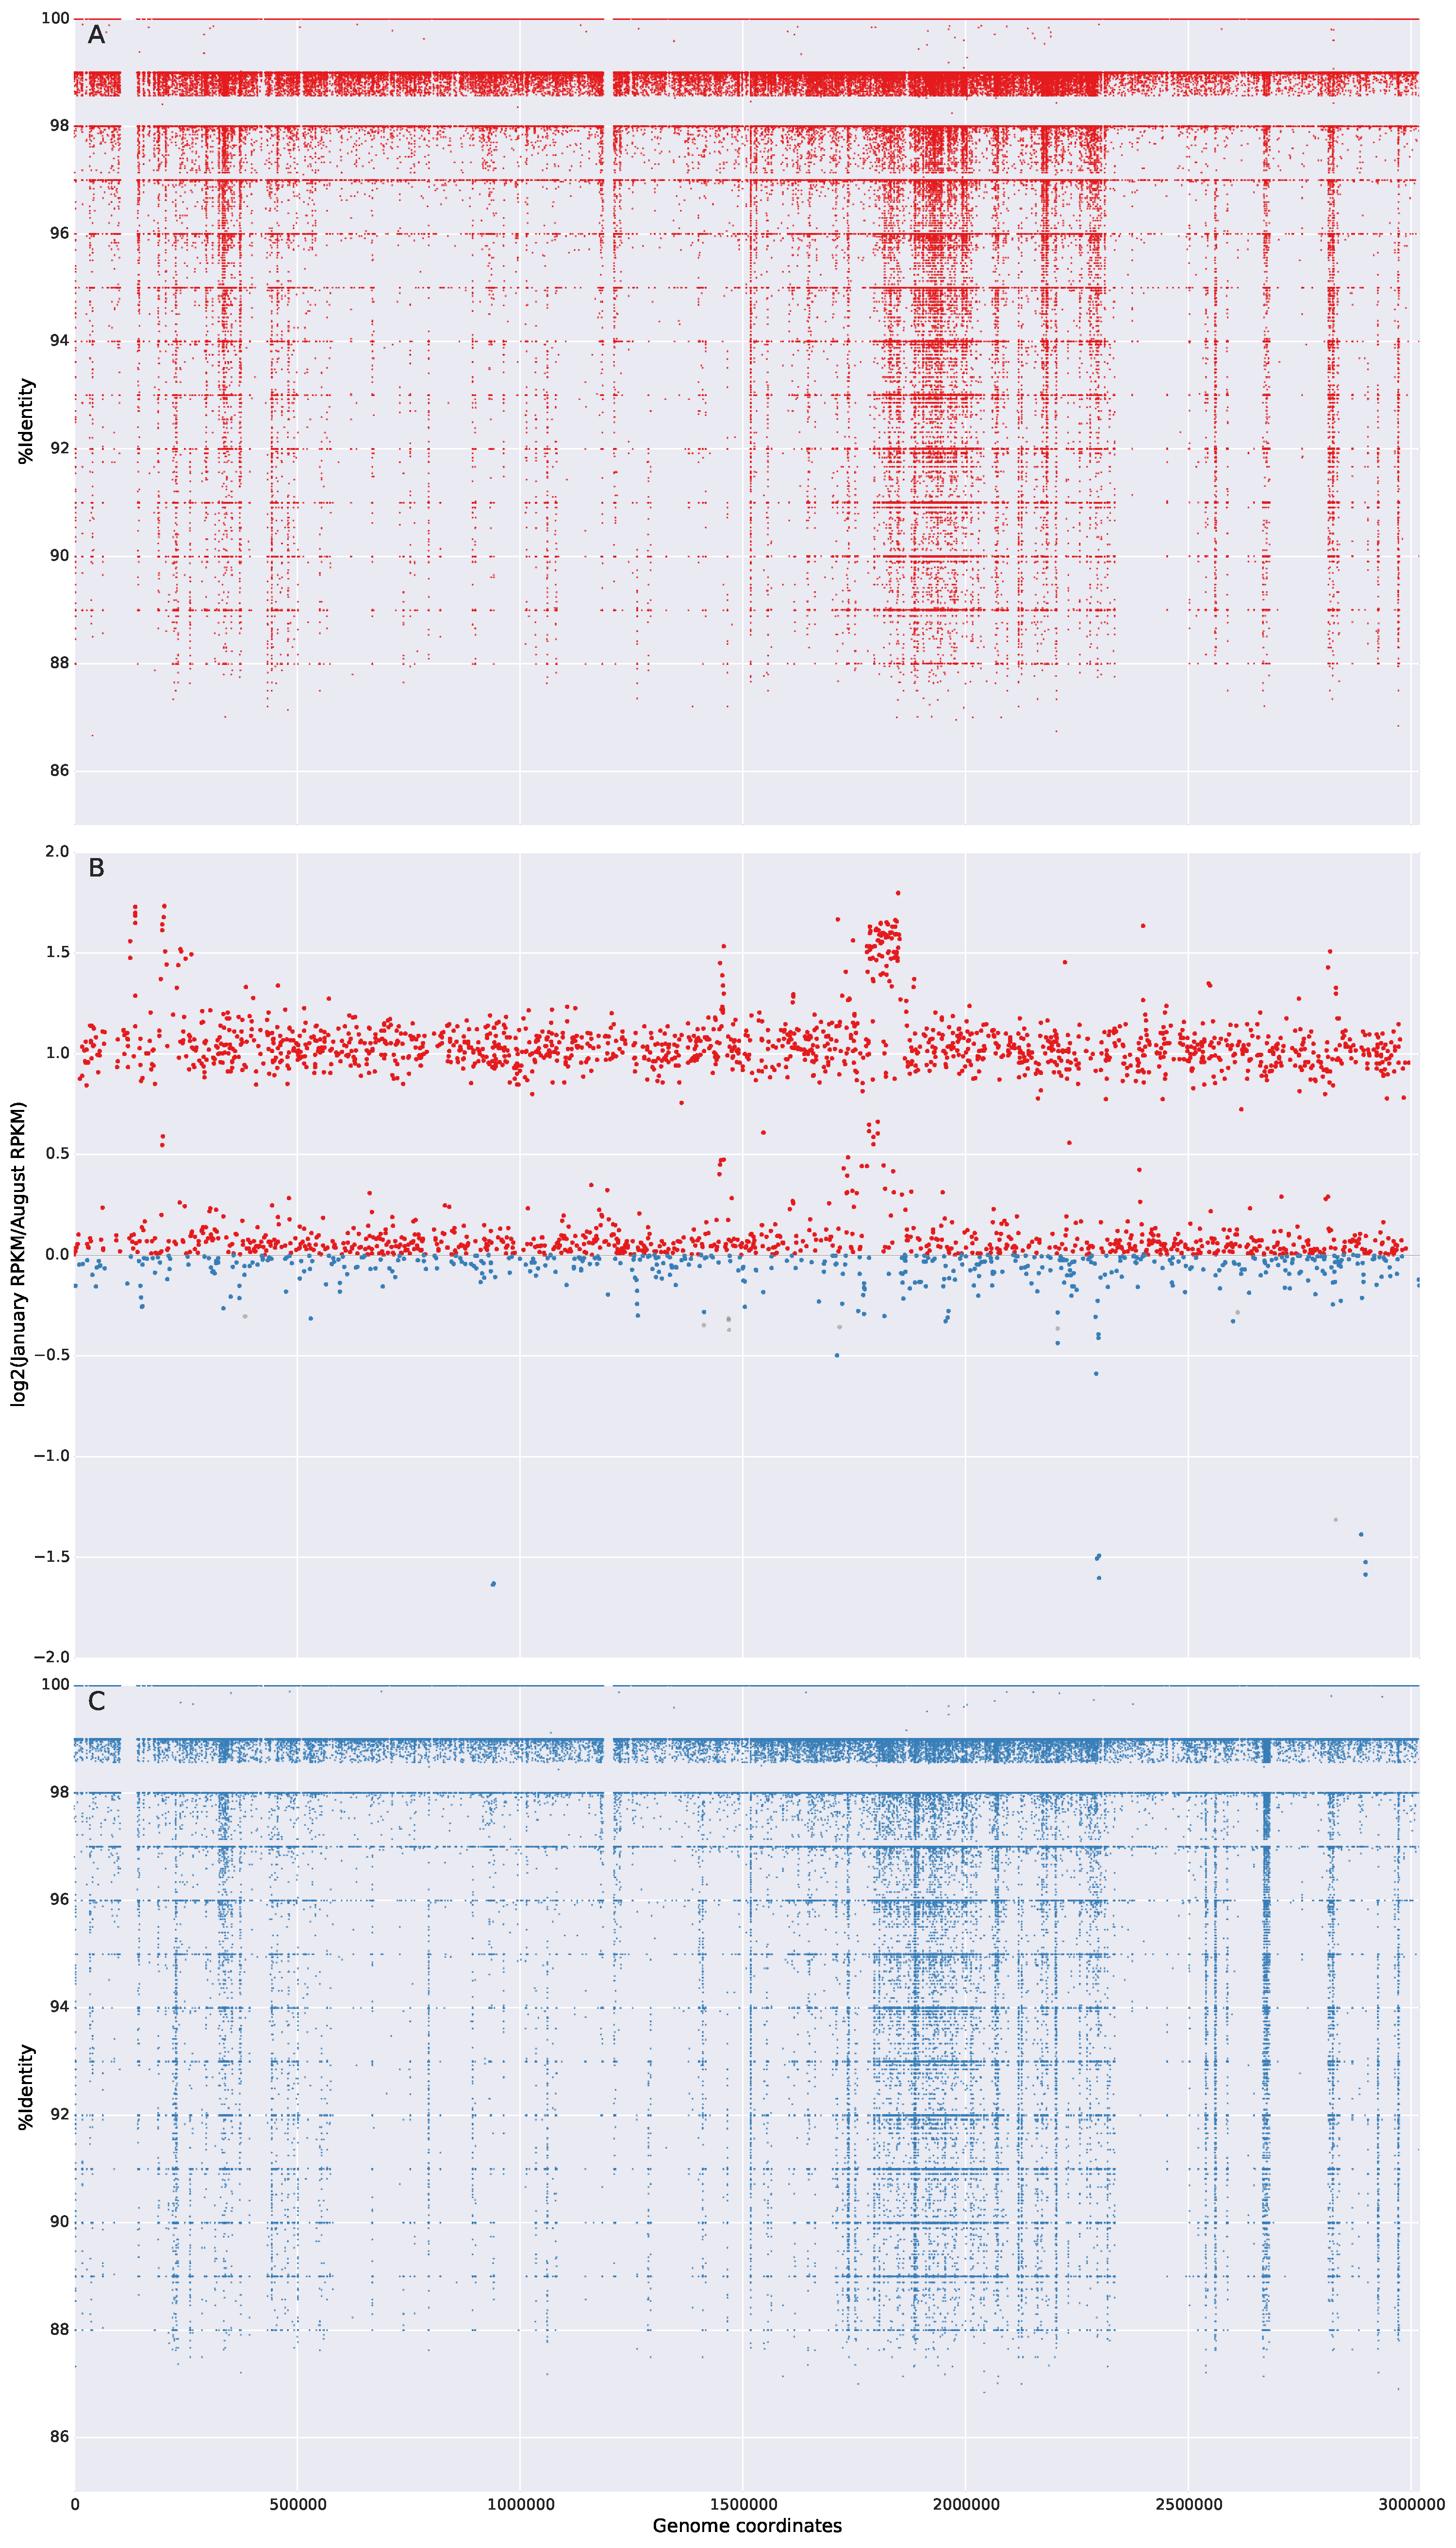
\includegraphics[width=\textwidth,height=0.8\textheight,keepaspectratio]{Chapter5/Figures/coverage_plots/J07HQX50_coverage.pdf}
  \caption{Coverage and gene abundance for J07HQX50. \textbf{A} and \textbf{C} shows reads recruited to the January and August genomes, respectively. \textbf{B} indicates the number of reads recruited to each individual gene, expressed as RPKM values, where the color indicates the sample from where the read originated (January vs. August.)}
  \label{J07HQXcoverage}
\end{figure}

\begin{figure}[!hbtp]
  \centering
  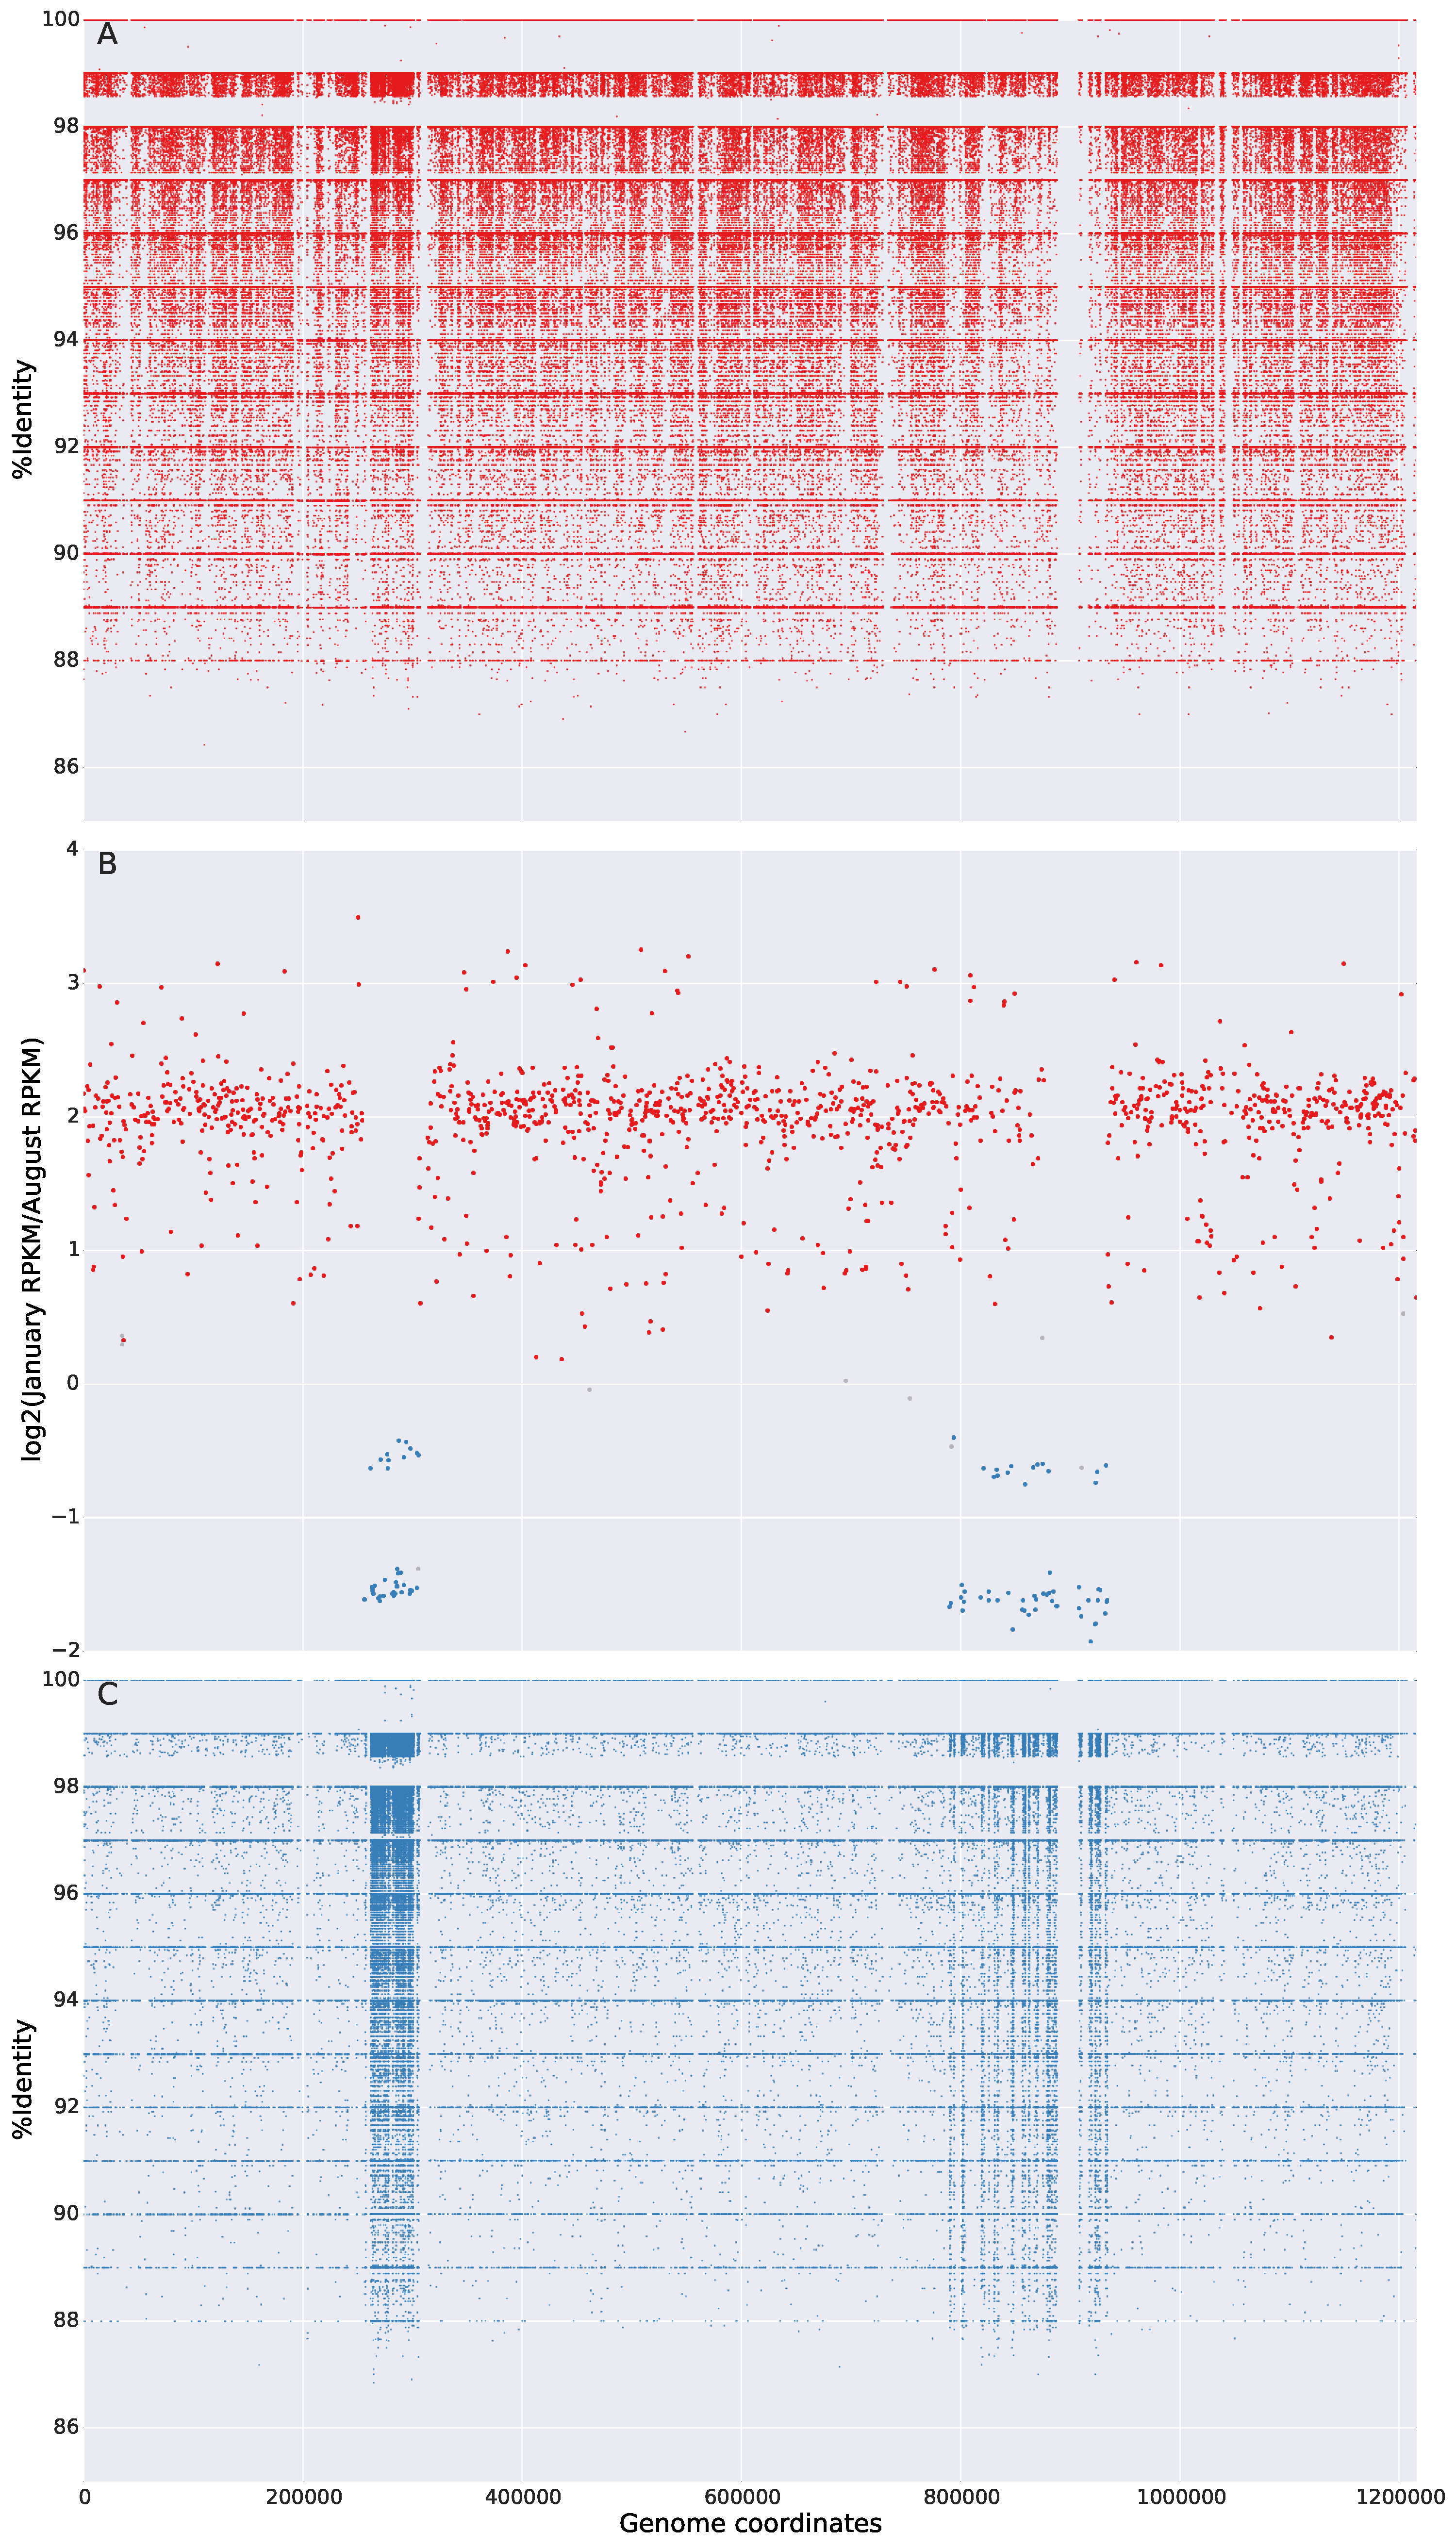
\includegraphics[width=\textwidth,height=0.8\textheight,keepaspectratio]{Chapter5/Figures/coverage_plots/J07AB56_coverage.pdf}
  \caption{Coverage and gene abundance for J07AB56. \textbf{A} and \textbf{C} shows reads recruited to the January and August genomes, respectively. \textbf{B} indicates the number of reads recruited to each individual gene, expressed as RPKM values, where the color indicates the sample from where the read originated (January vs. August.)}
  \label{J07AB56coverage}
\end{figure}

\begin{figure}[!hbtp]
  \centering
  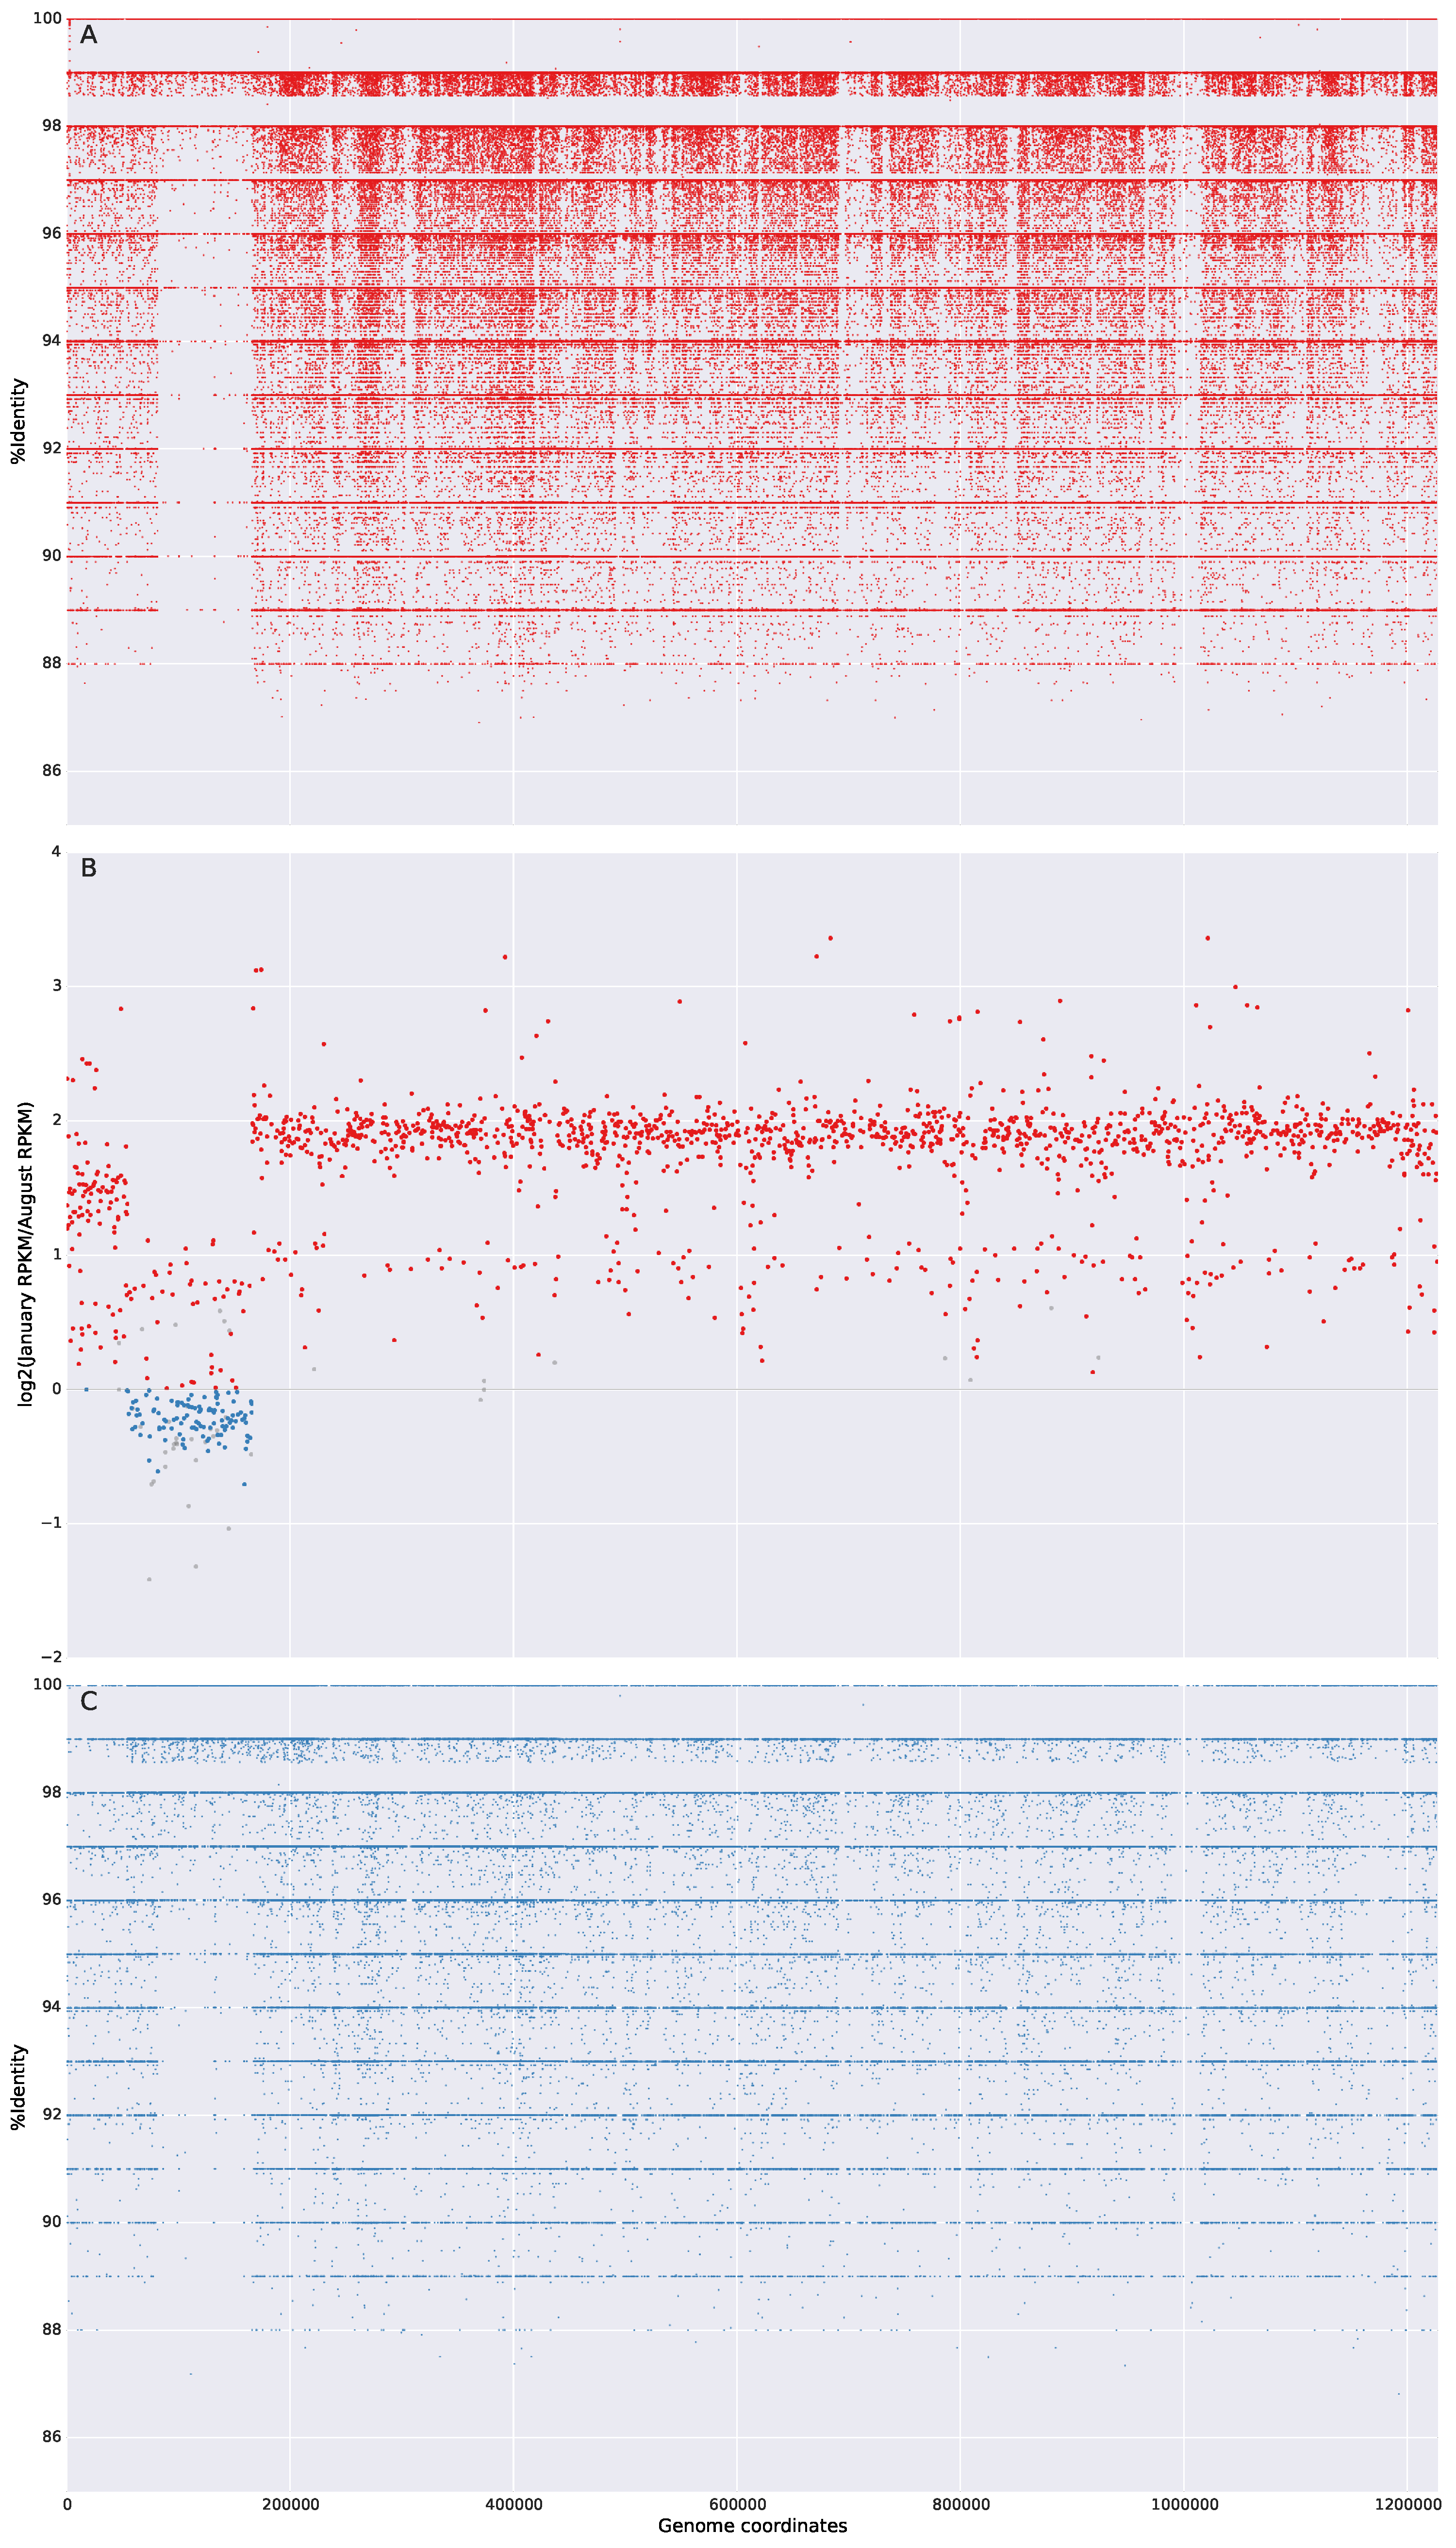
\includegraphics[width=\textwidth,height=0.8\textheight,keepaspectratio]{Chapter5/Figures/coverage_plots/J07AB43_coverage.pdf}
  \caption{Coverage and gene abundance for J07AB43. \textbf{A} and \textbf{C} shows reads recruited to the January and August genomes, respectively. \textbf{B} indicates the number of reads recruited to each individual gene, expressed as RPKM values, where the color indicates the sample from where the read originated (January vs. August.)}
  \label{J07AB43ccoverage}
\end{figure}

\begin{figure}[!hbtp]
  \centering
  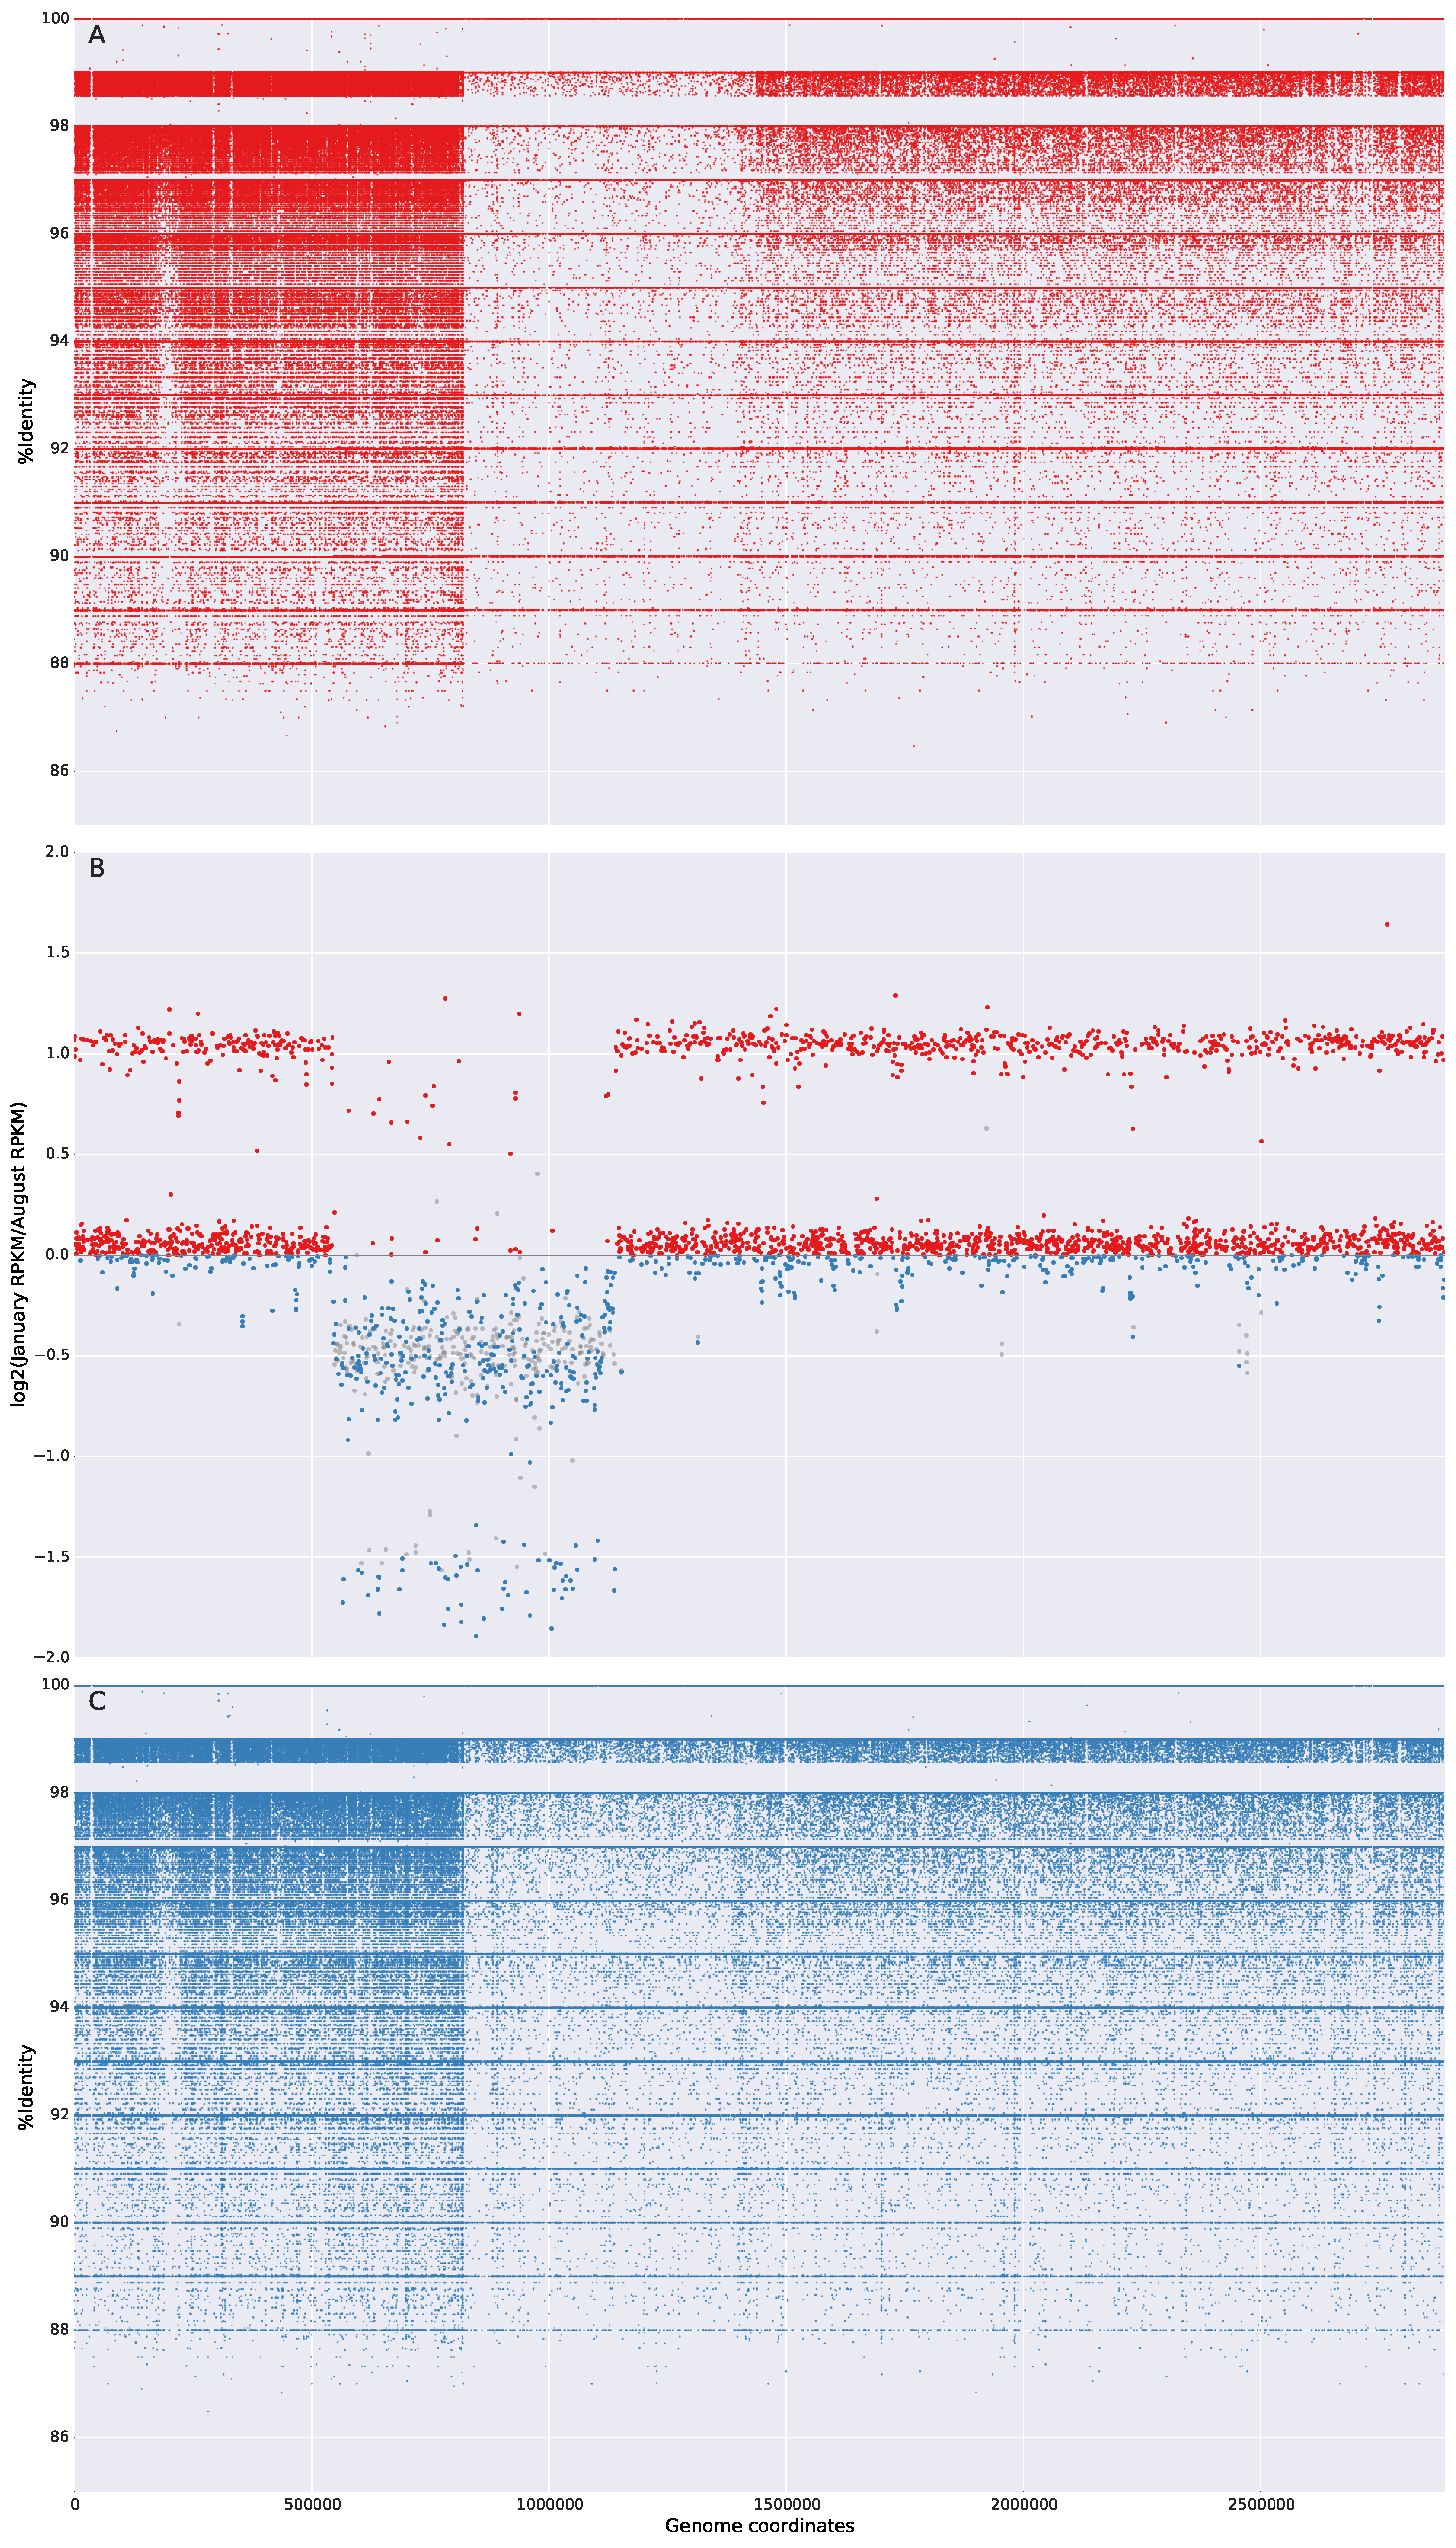
\includegraphics[width=\textwidth,height=0.8\textheight,keepaspectratio]{Chapter5/Figures/coverage_plots/J07HN4_coverage.pdf}
  \caption{Coverage and gene abundance for J07HN4. \textbf{A} and \textbf{C} shows reads recruited to the January and August genomes, respectively. \textbf{B} indicates the number of reads recruited to each individual gene, expressed as RPKM values, where the color indicates the sample from where the read originated (January vs. August.)}
  \label{J07HN4coverage}
\end{figure}

\begin{figure}[!hbtp]
  \centering
  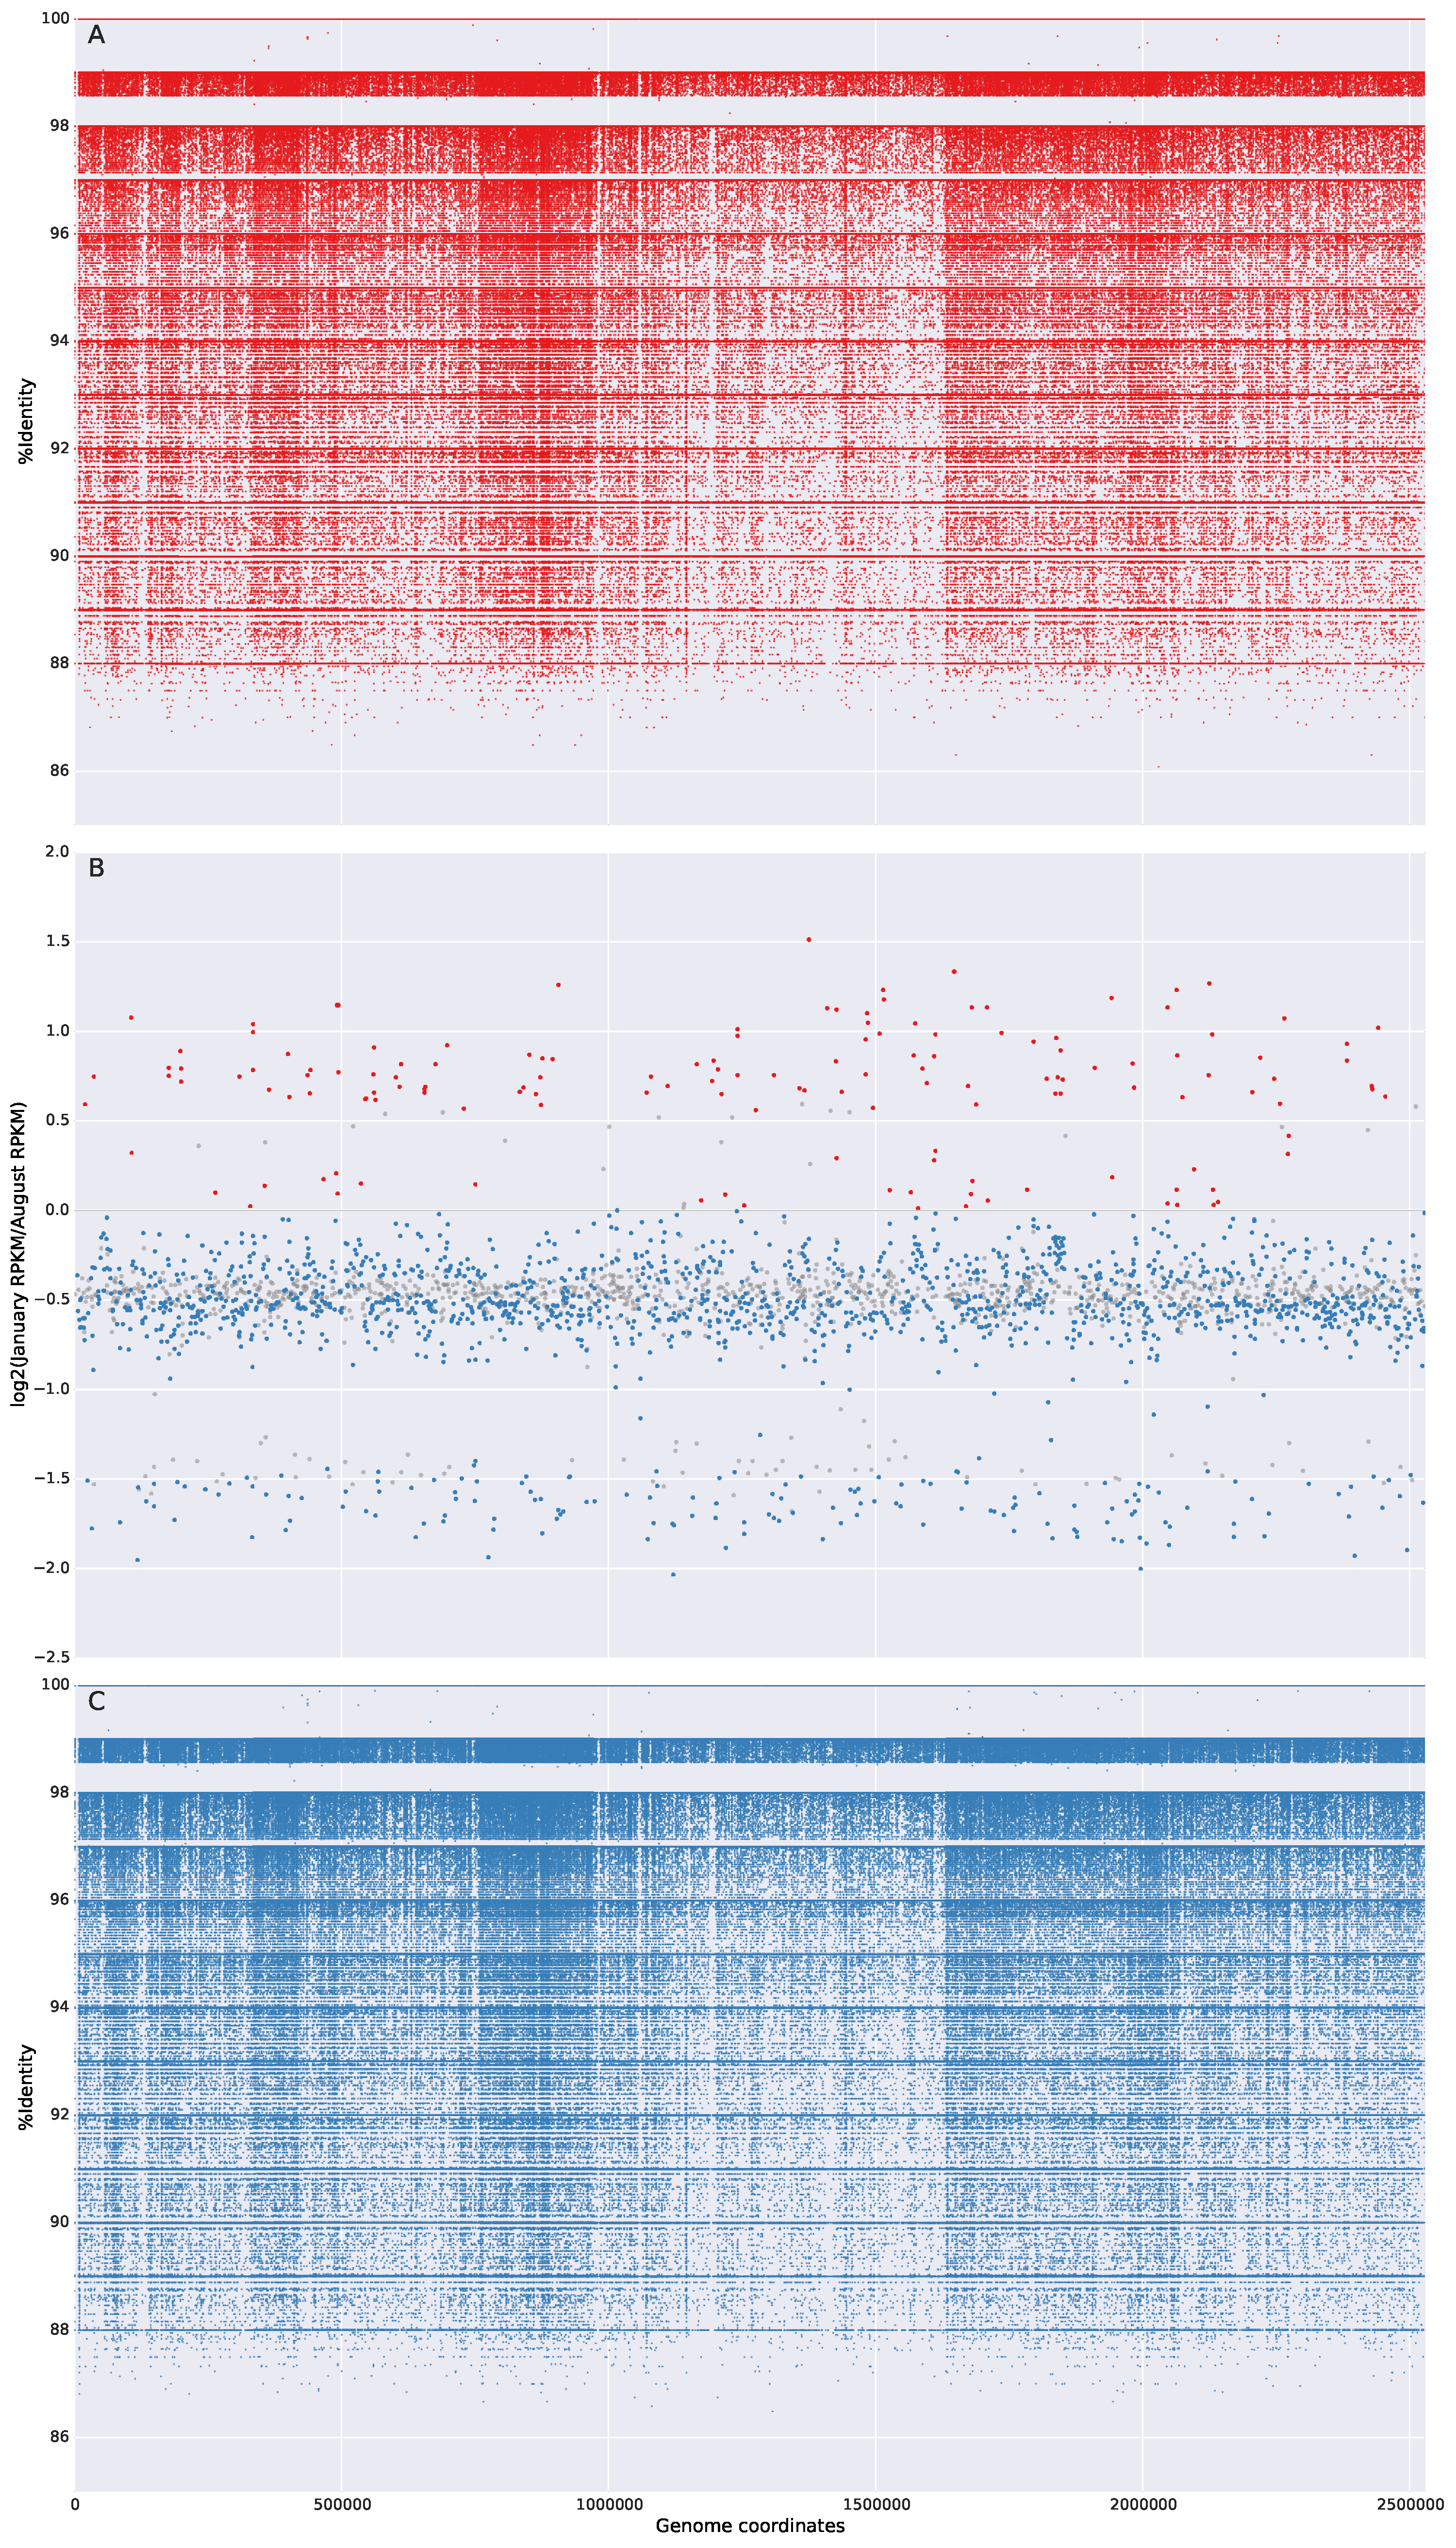
\includegraphics[width=\textwidth,height=0.8\textheight,keepaspectratio]{Chapter5/Figures/coverage_plots/J07HN6_coverage.pdf}
  \caption{Coverage and gene abundance for J07HN6. \textbf{A} and \textbf{C} shows reads recruited to the January and August genomes, respectively. \textbf{B} indicates the number of reads recruited to each individual gene, expressed as RPKM values, where the color indicates the sample from where the read originated (January vs. August.)}
  \label{J07HN6coverage}
\end{figure}

\begin{figure}[!hbtp]
  \centering
  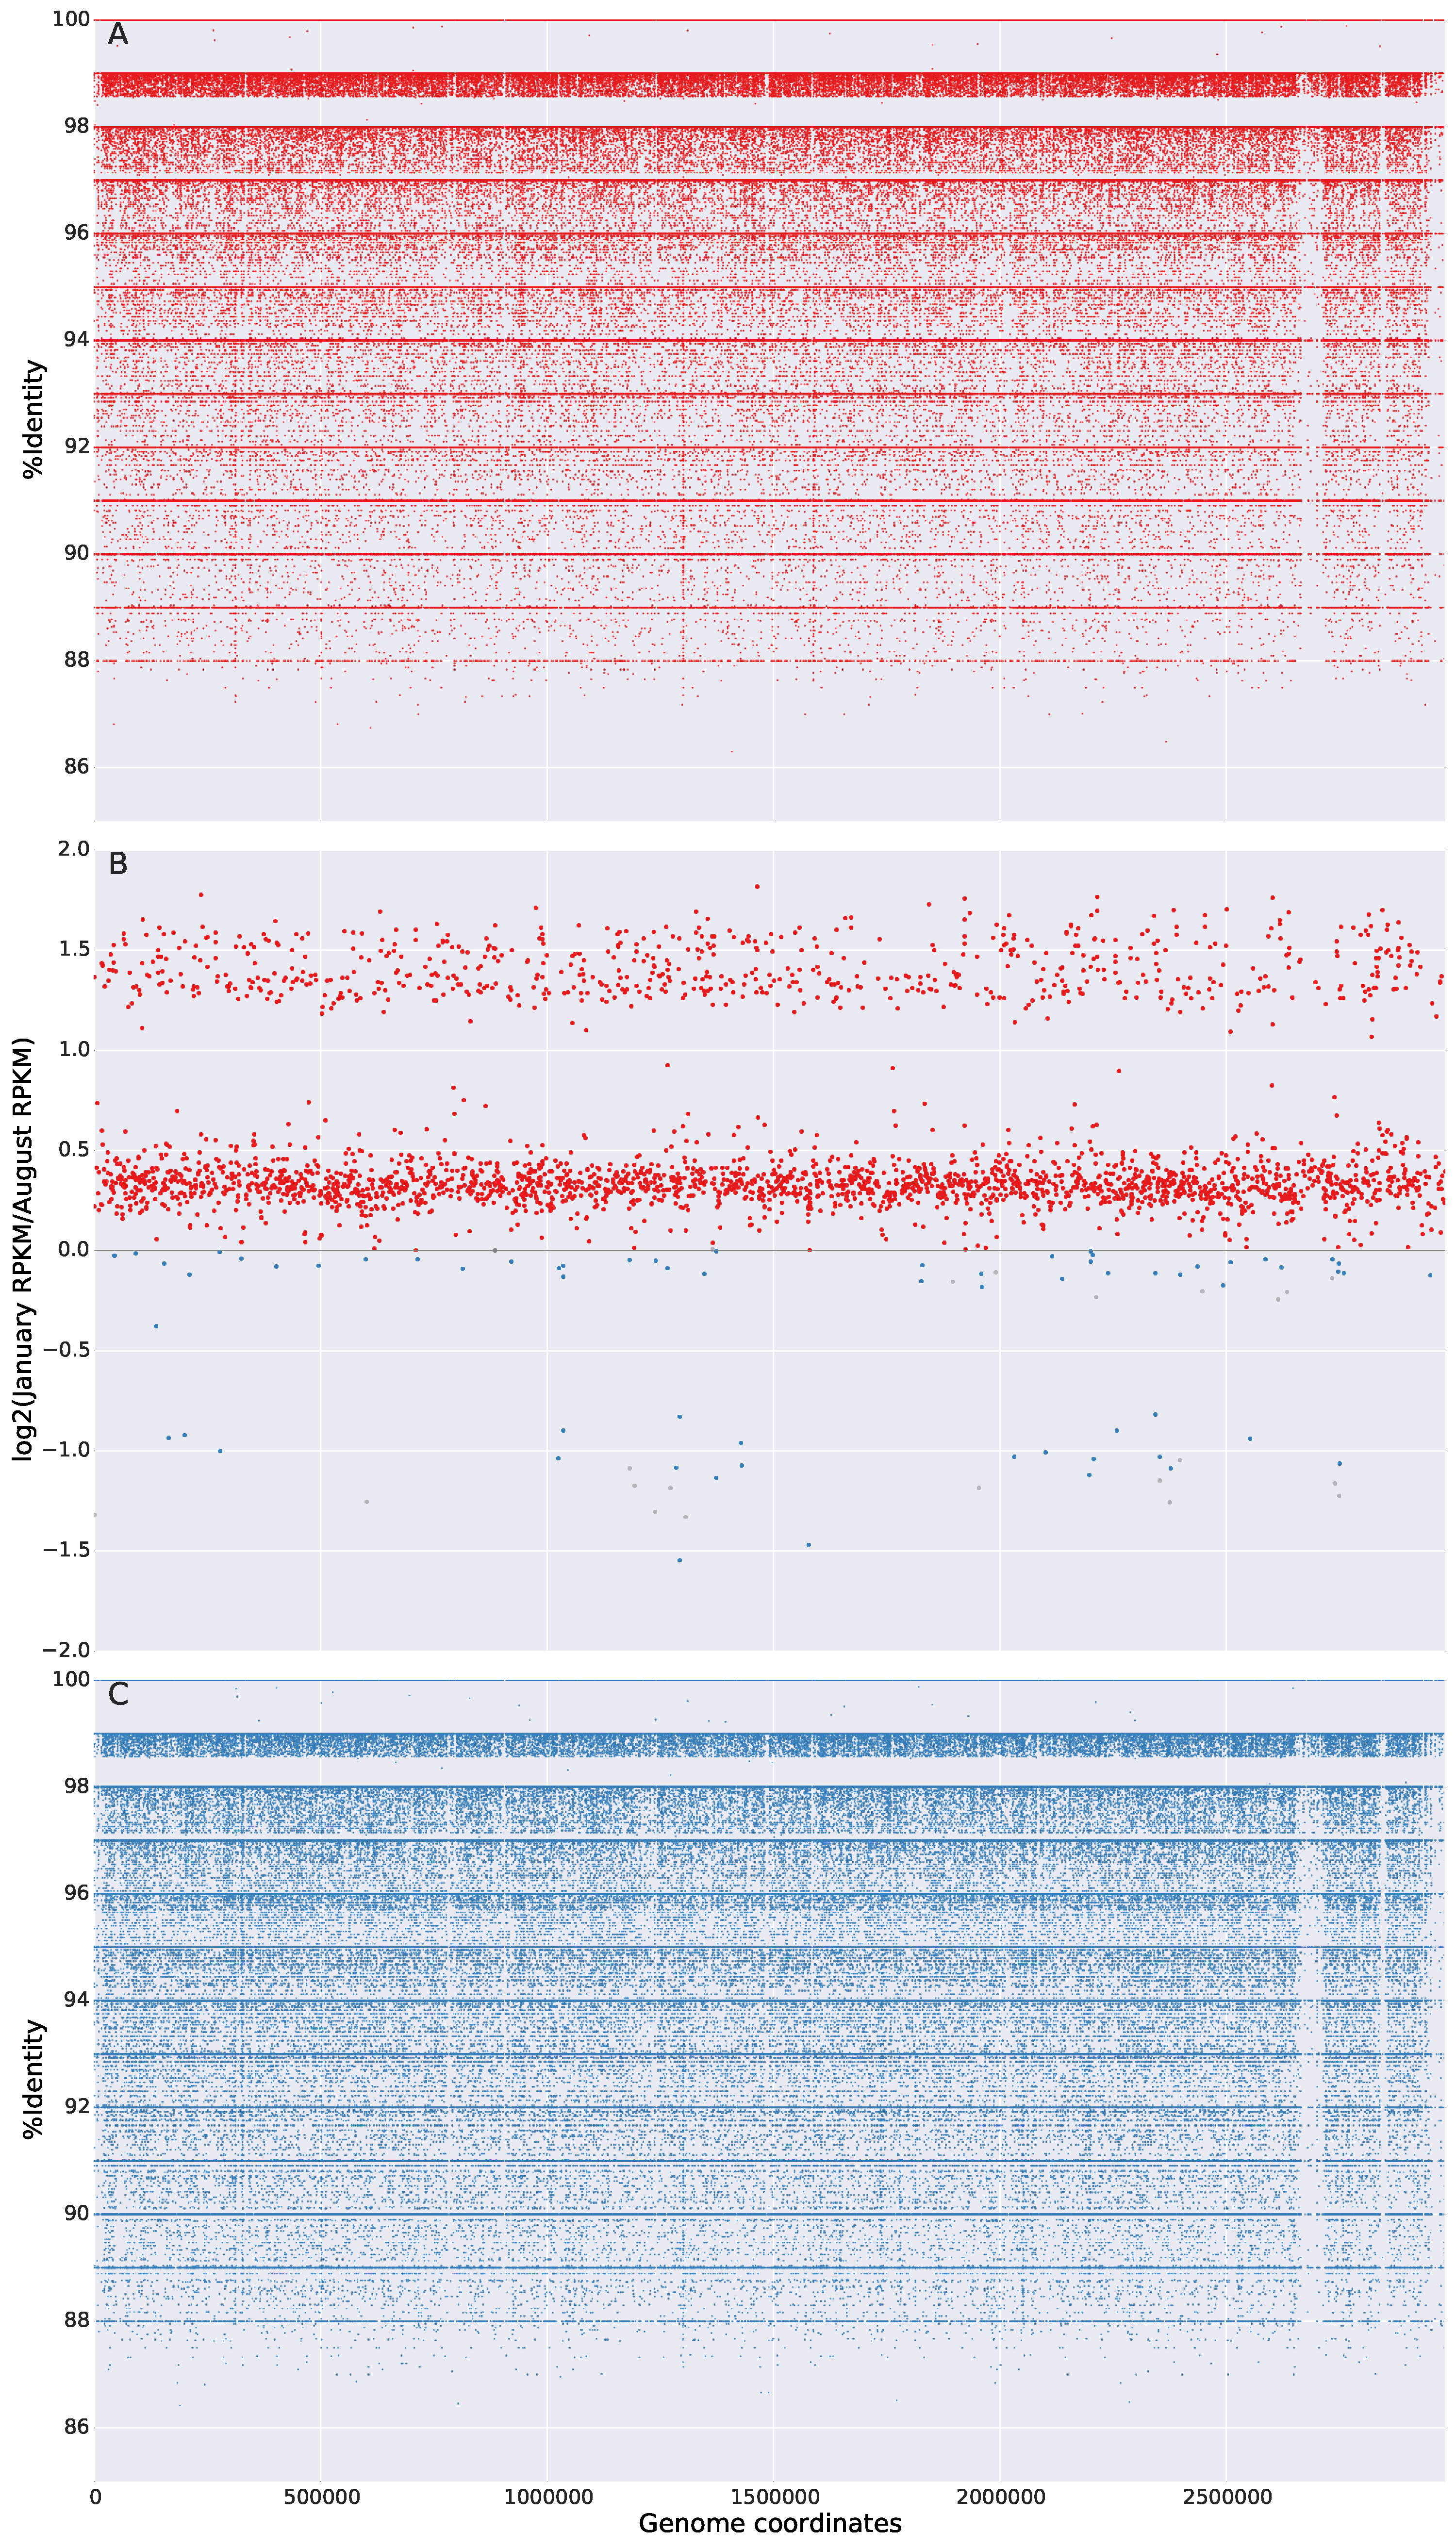
\includegraphics[width=\textwidth,height=0.8\textheight,keepaspectratio]{Chapter5/Figures/coverage_plots/J07HX64_coverage.pdf}
  \caption{Coverage and gene abundance for J07HN64. \textbf{A} and \textbf{C} shows reads recruited to the January and August genomes, respectively. \textbf{B} indicates the number of reads recruited to each individual gene, expressed as RPKM values, where the color indicates the sample from where the read originated (January vs. August.)}
  \label{J07HN64coverage}
\end{figure}

\begin{figure}[!hbtp]
  \centering
  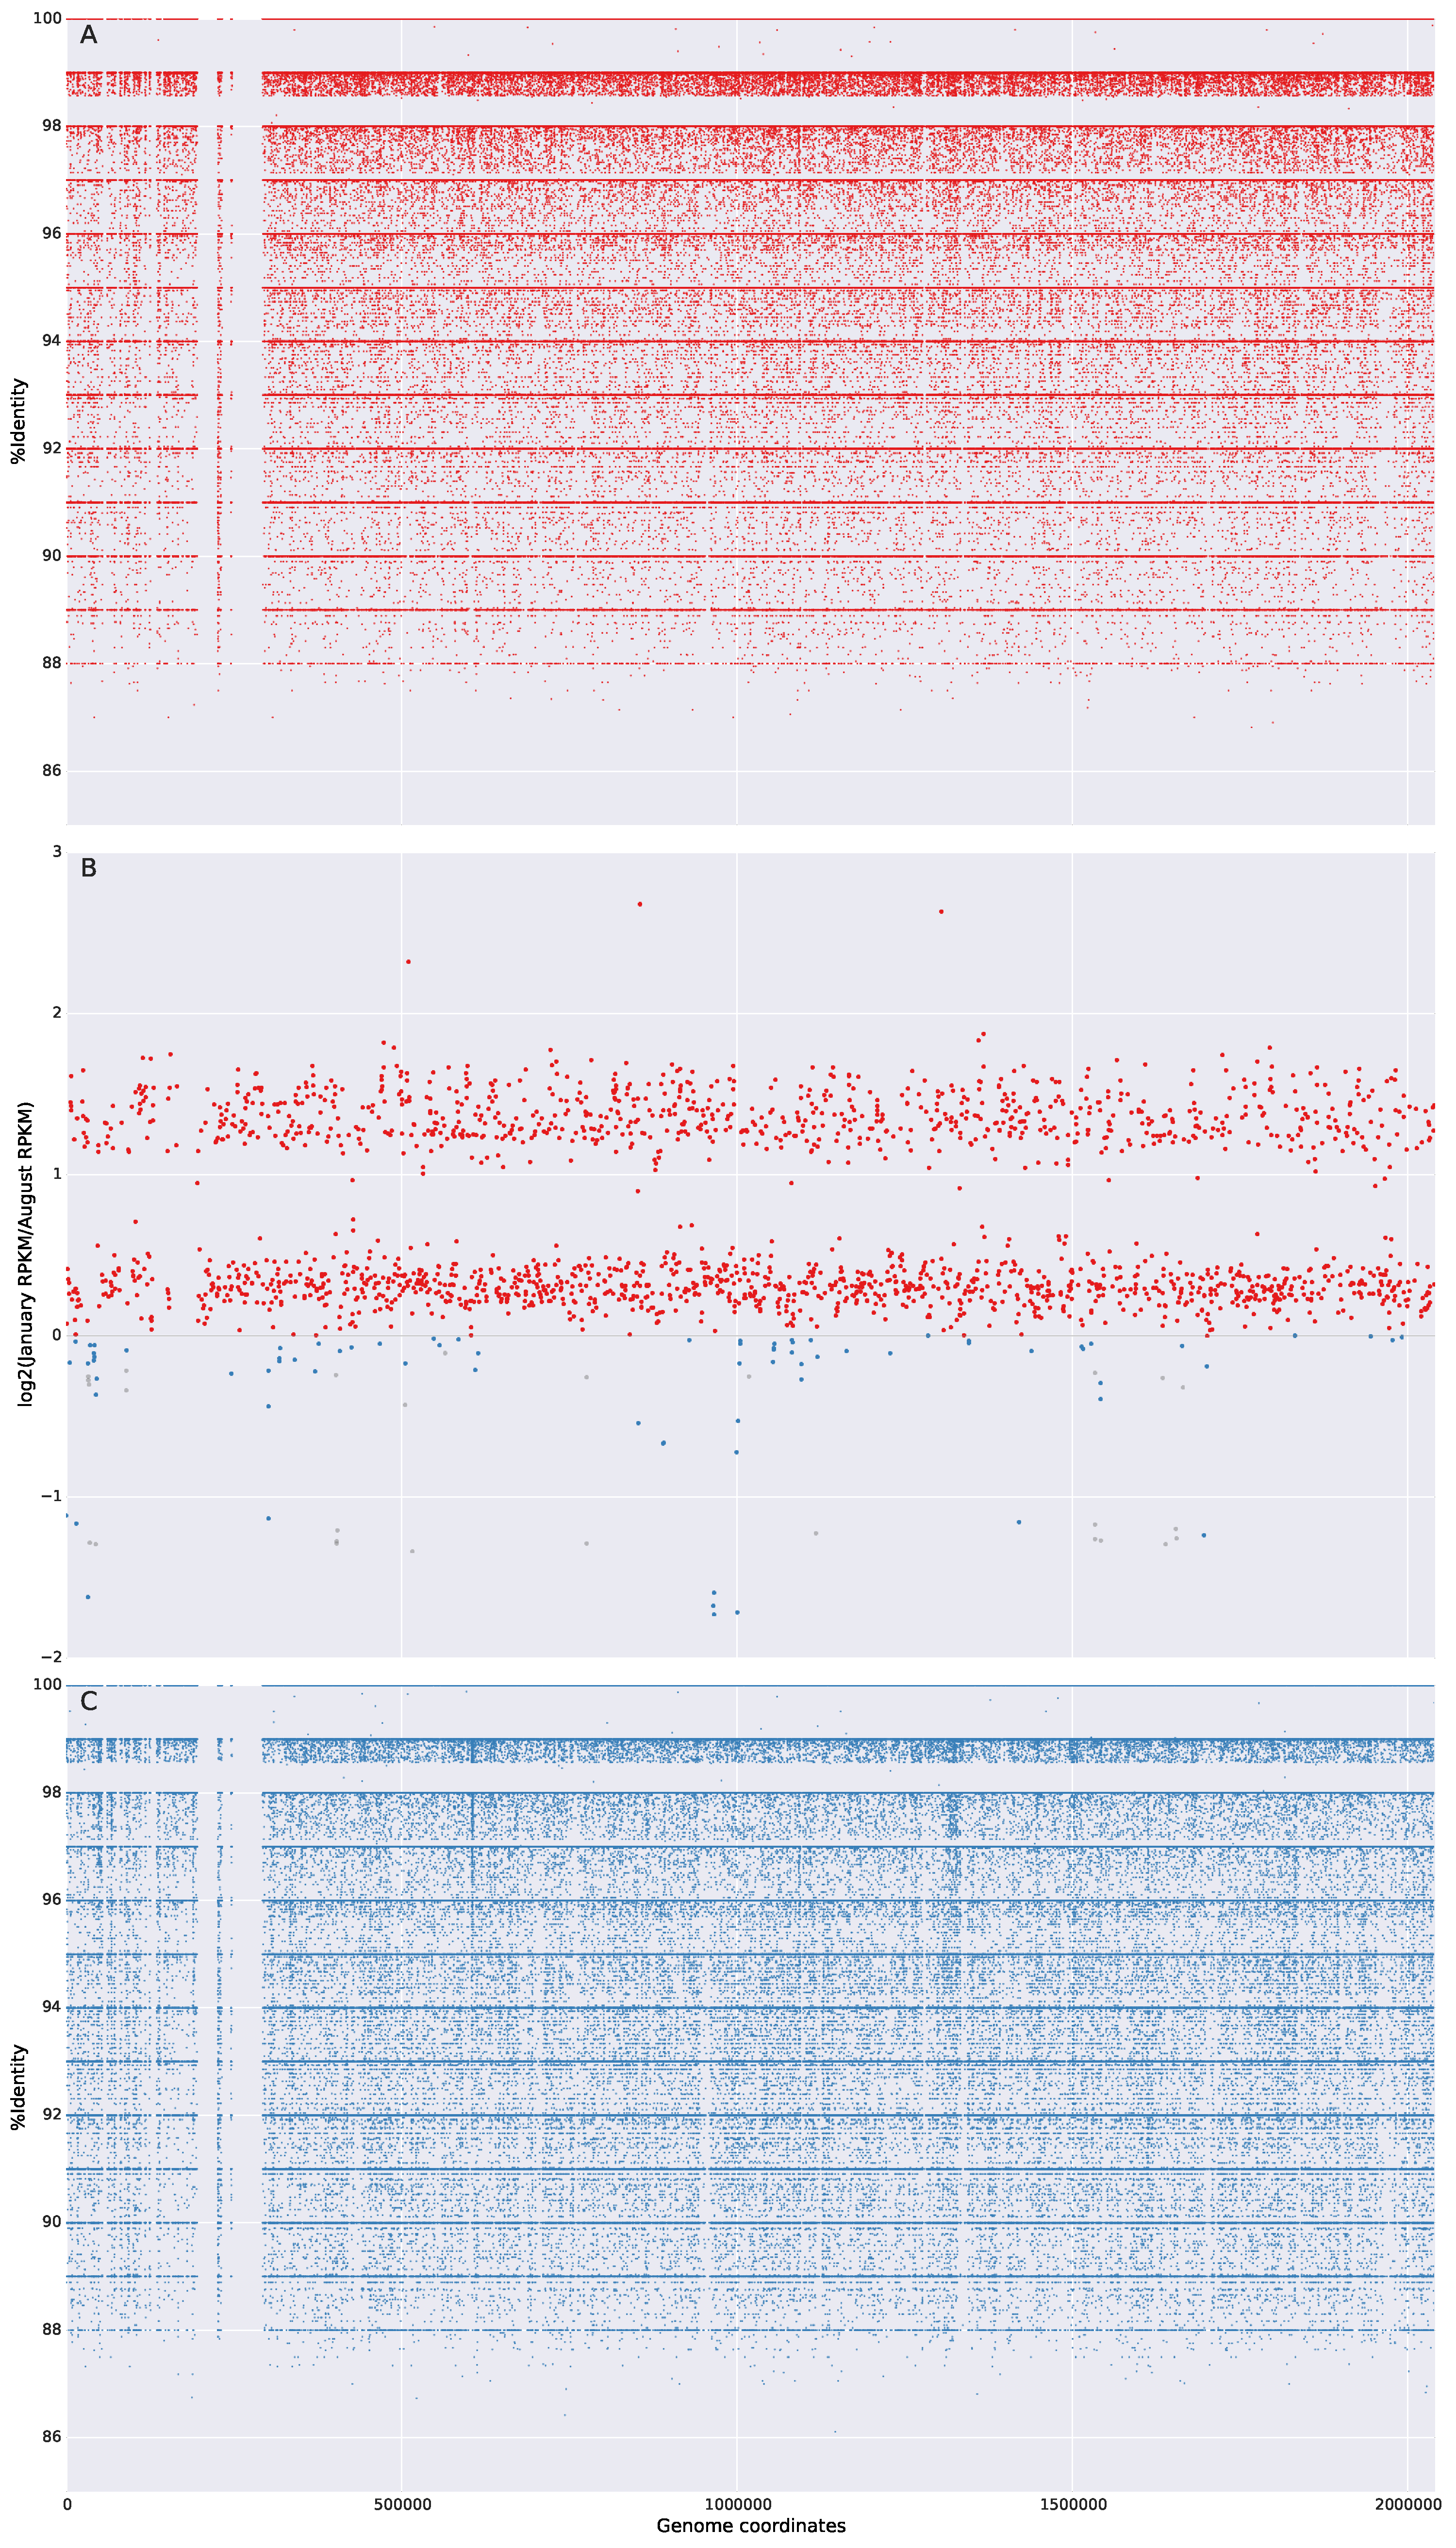
\includegraphics[width=\textwidth,height=0.8\textheight,keepaspectratio]{Chapter5/Figures/coverage_plots/J07HX5_coverage.pdf}
  \caption{Coverage and gene abundance for J07HX5. \textbf{A} and \textbf{C} shows reads recruited to the January and August genomes, respectively. \textbf{B} indicates the number of reads recruited to each individual gene, expressed as RPKM values, where the color indicates the sample from where the read originated (January vs. August.)}
  \label{J07HX5coverage}
\end{figure}

\begin{figure}[!hbtp]
  \centering
  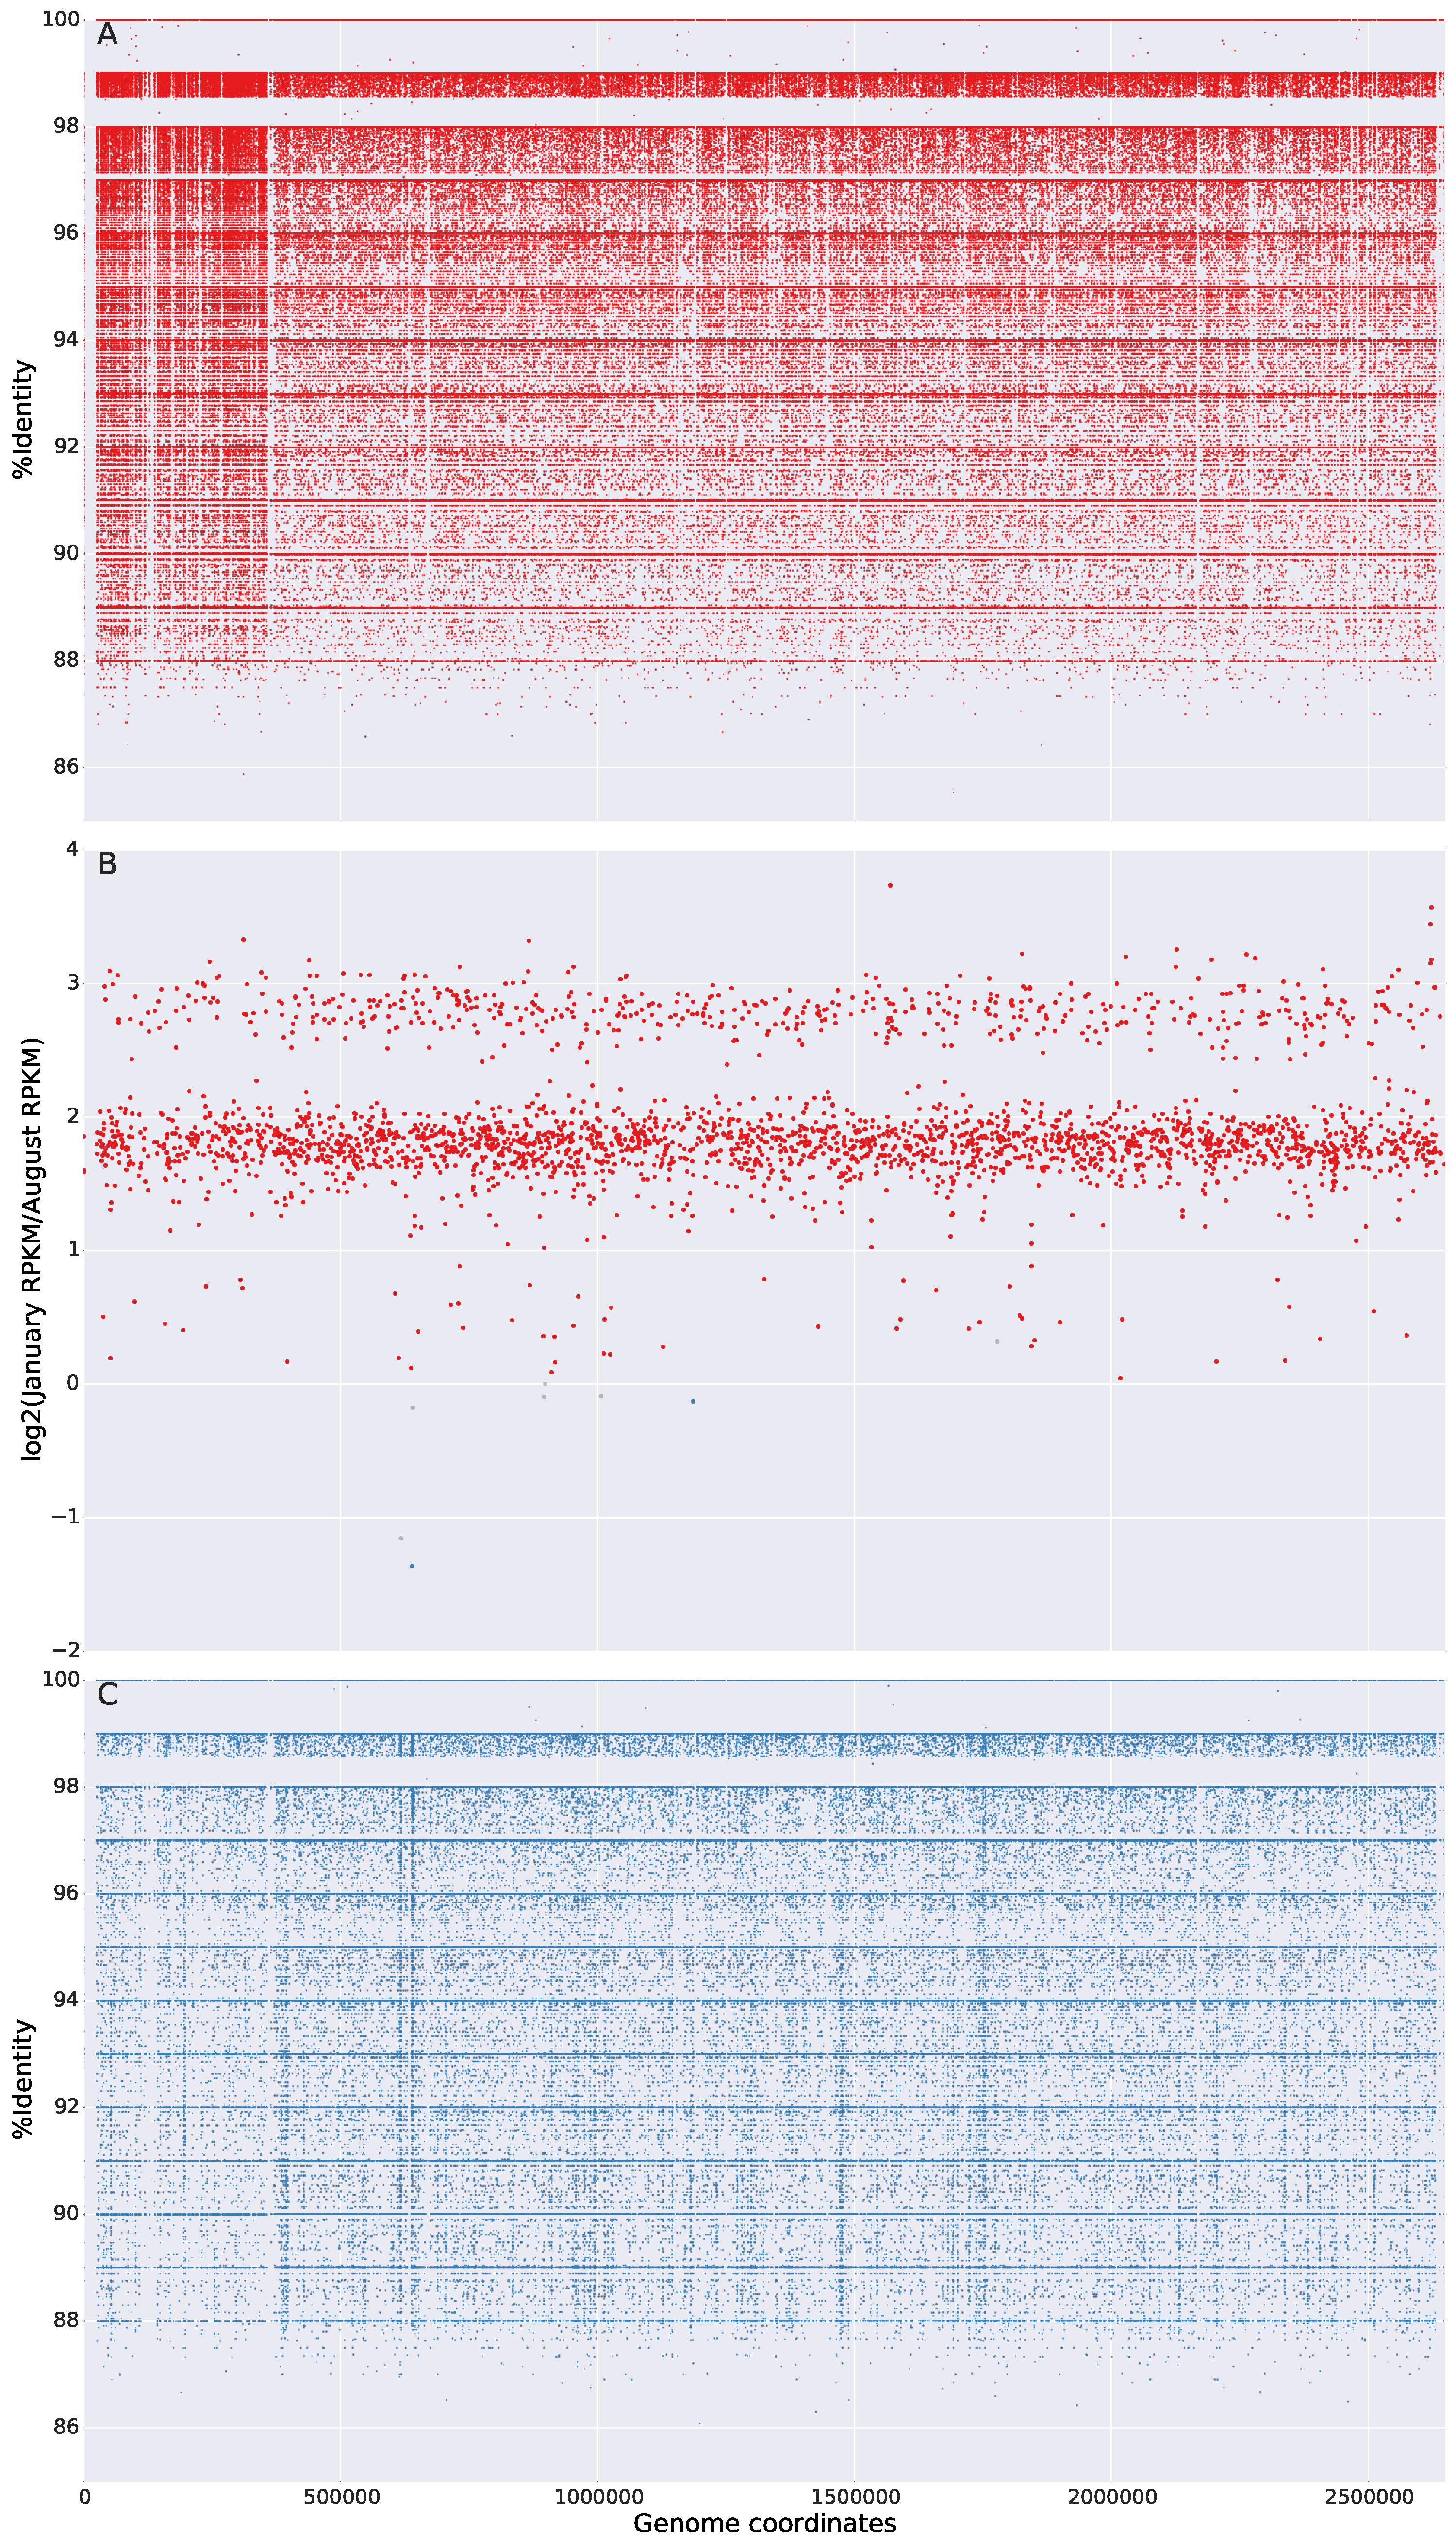
\includegraphics[width=\textwidth,height=0.8\textheight,keepaspectratio]{Chapter5/Figures/coverage_plots/J07HB67_coverage.pdf}
  \caption{Coverage and gene abundance for J07HB67. \textbf{A} and \textbf{C} shows reads recruited to the January and August genomes, respectively. \textbf{B} indicates the number of reads recruited to each individual gene, expressed as RPKM values, where the color indicates the sample from where the read originated (January vs. August.)}
  \label{J07HB67coverage}
\end{figure}

\begin{figure}[!hbtp]
  \centering
  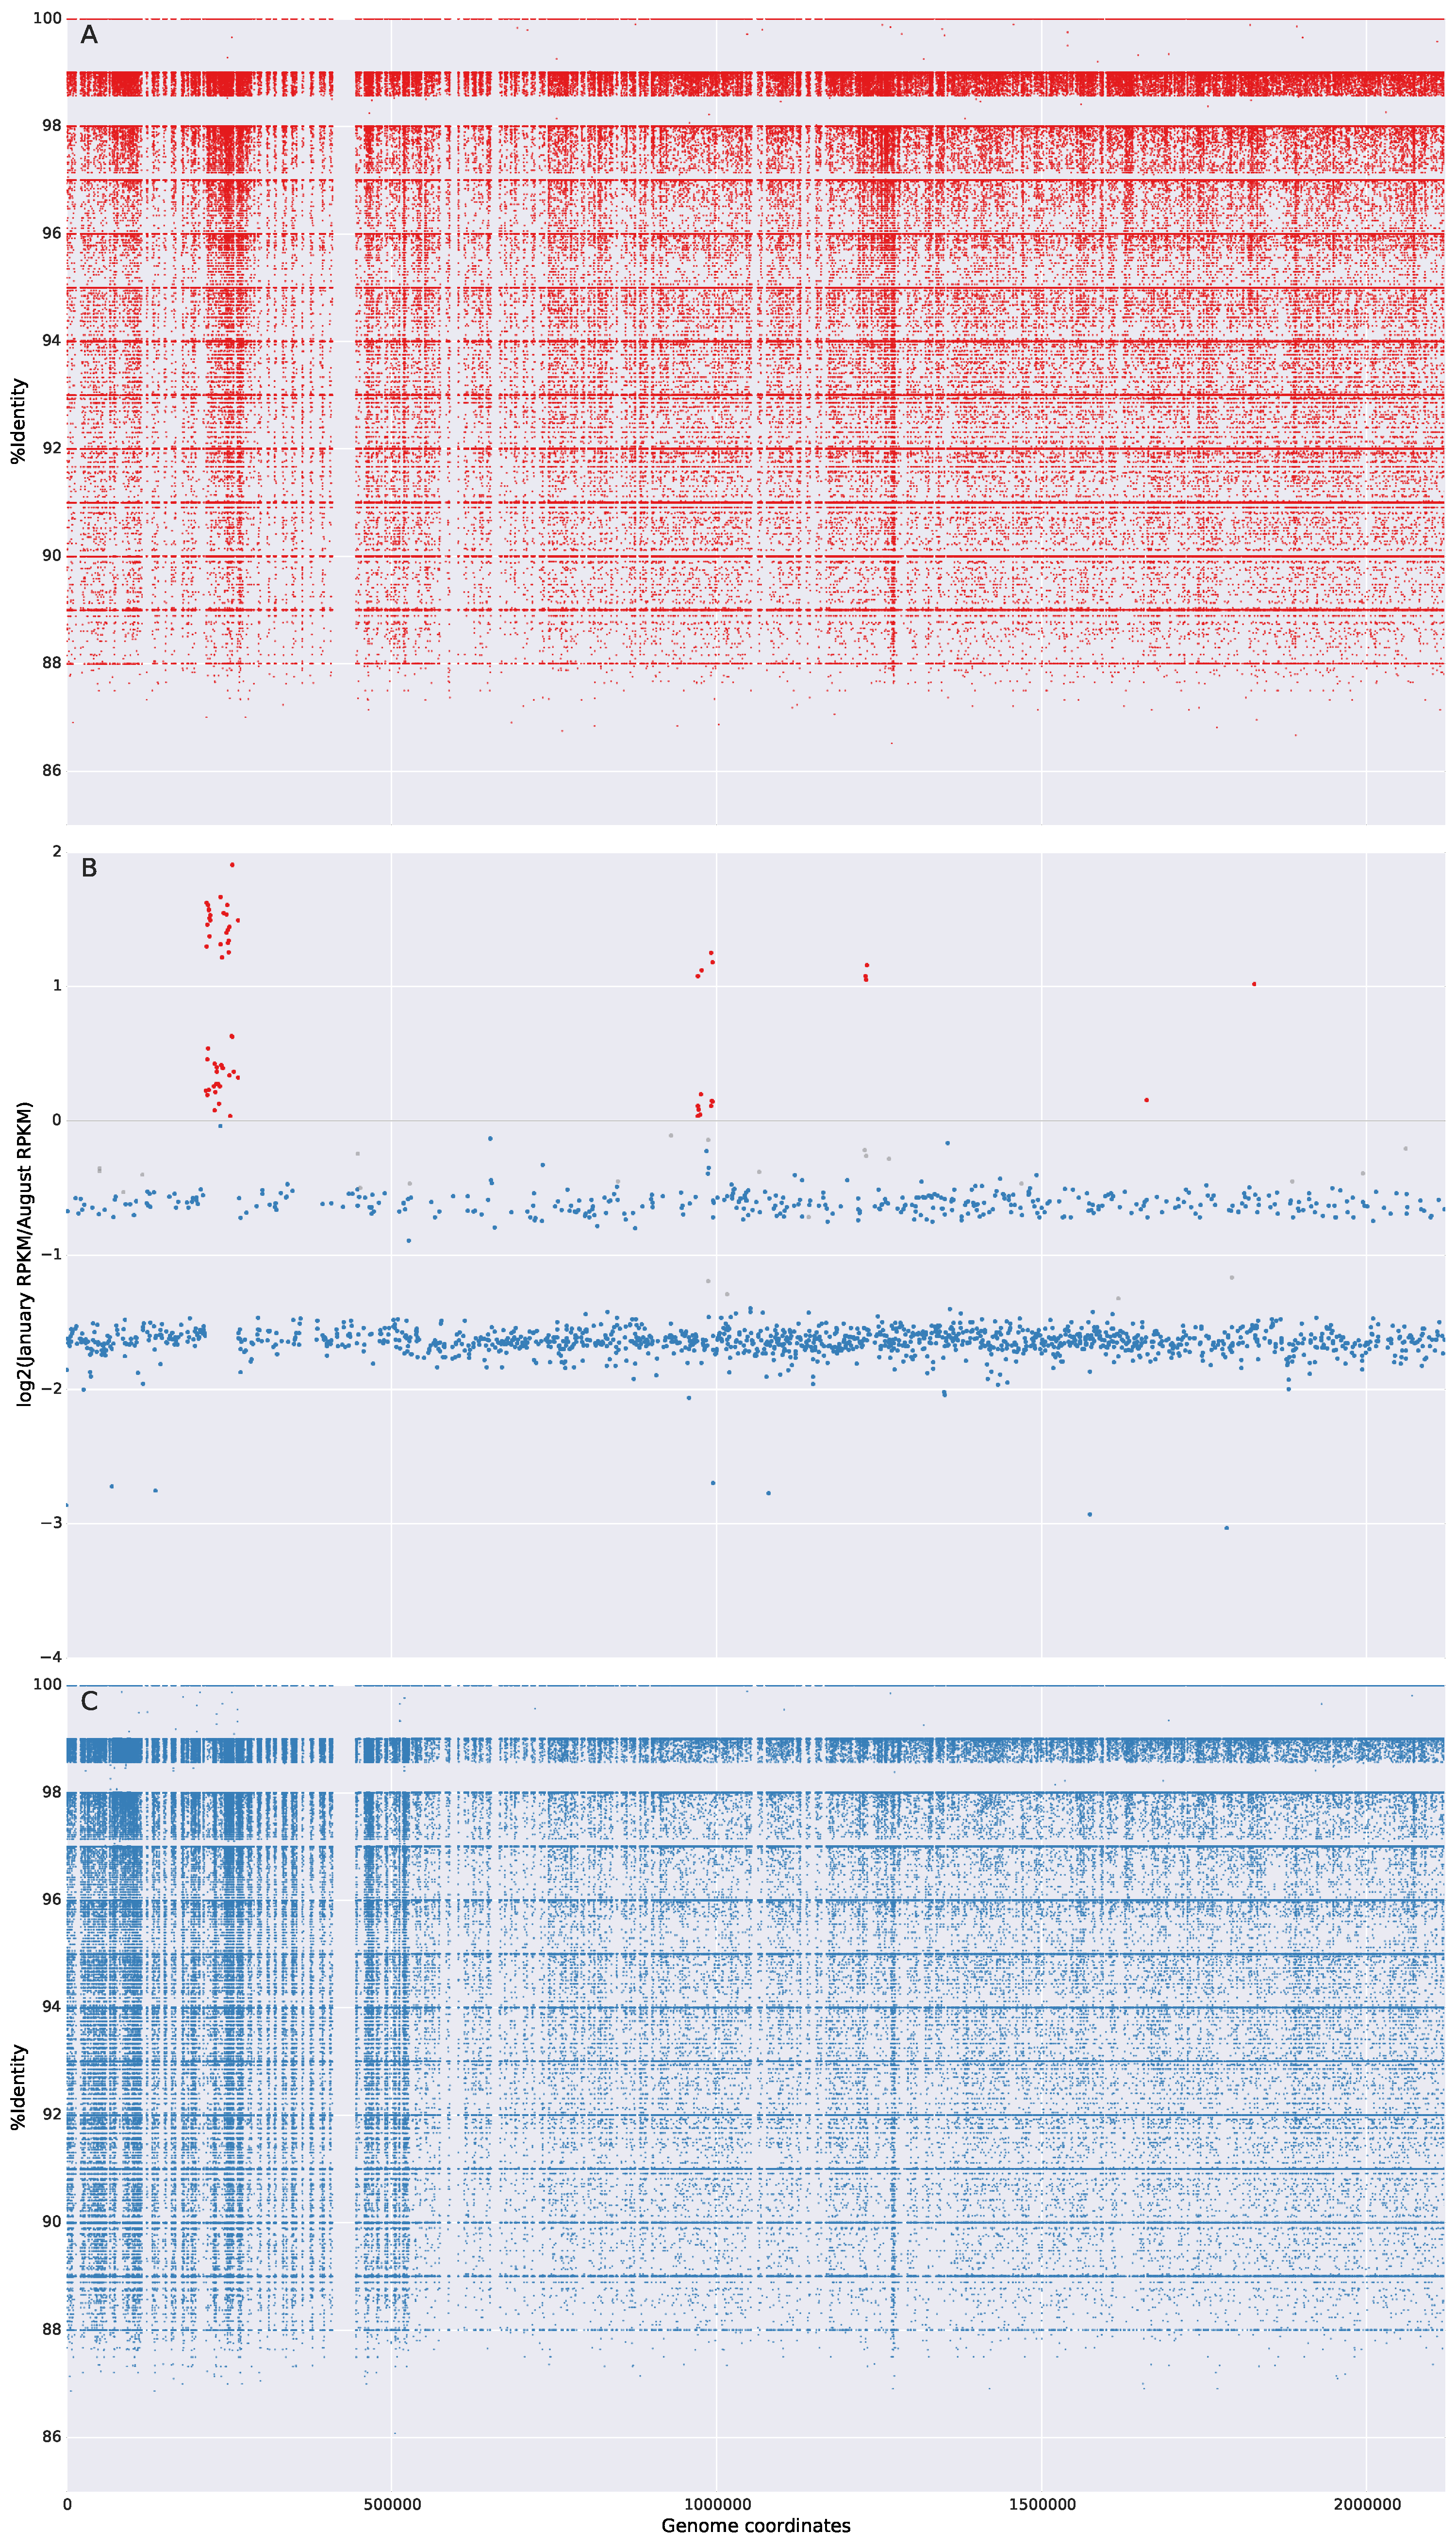
\includegraphics[width=\textwidth,height=0.8\textheight,keepaspectratio]{Chapter5/Figures/coverage_plots/J07HR59_coverage.pdf}
  \caption{Coverage and gene abundance for J07HR59. \textbf{A} and \textbf{C} shows reads recruited to the January and August genomes, respectively. \textbf{B} indicates the number of reads recruited to each individual gene, expressed as RPKM values, where the color indicates the sample from where the read originated (January vs. August.)}
  \label{J07HR59coverage}
\end{figure}

\begin{figure}[!hbtp]
  \centering
  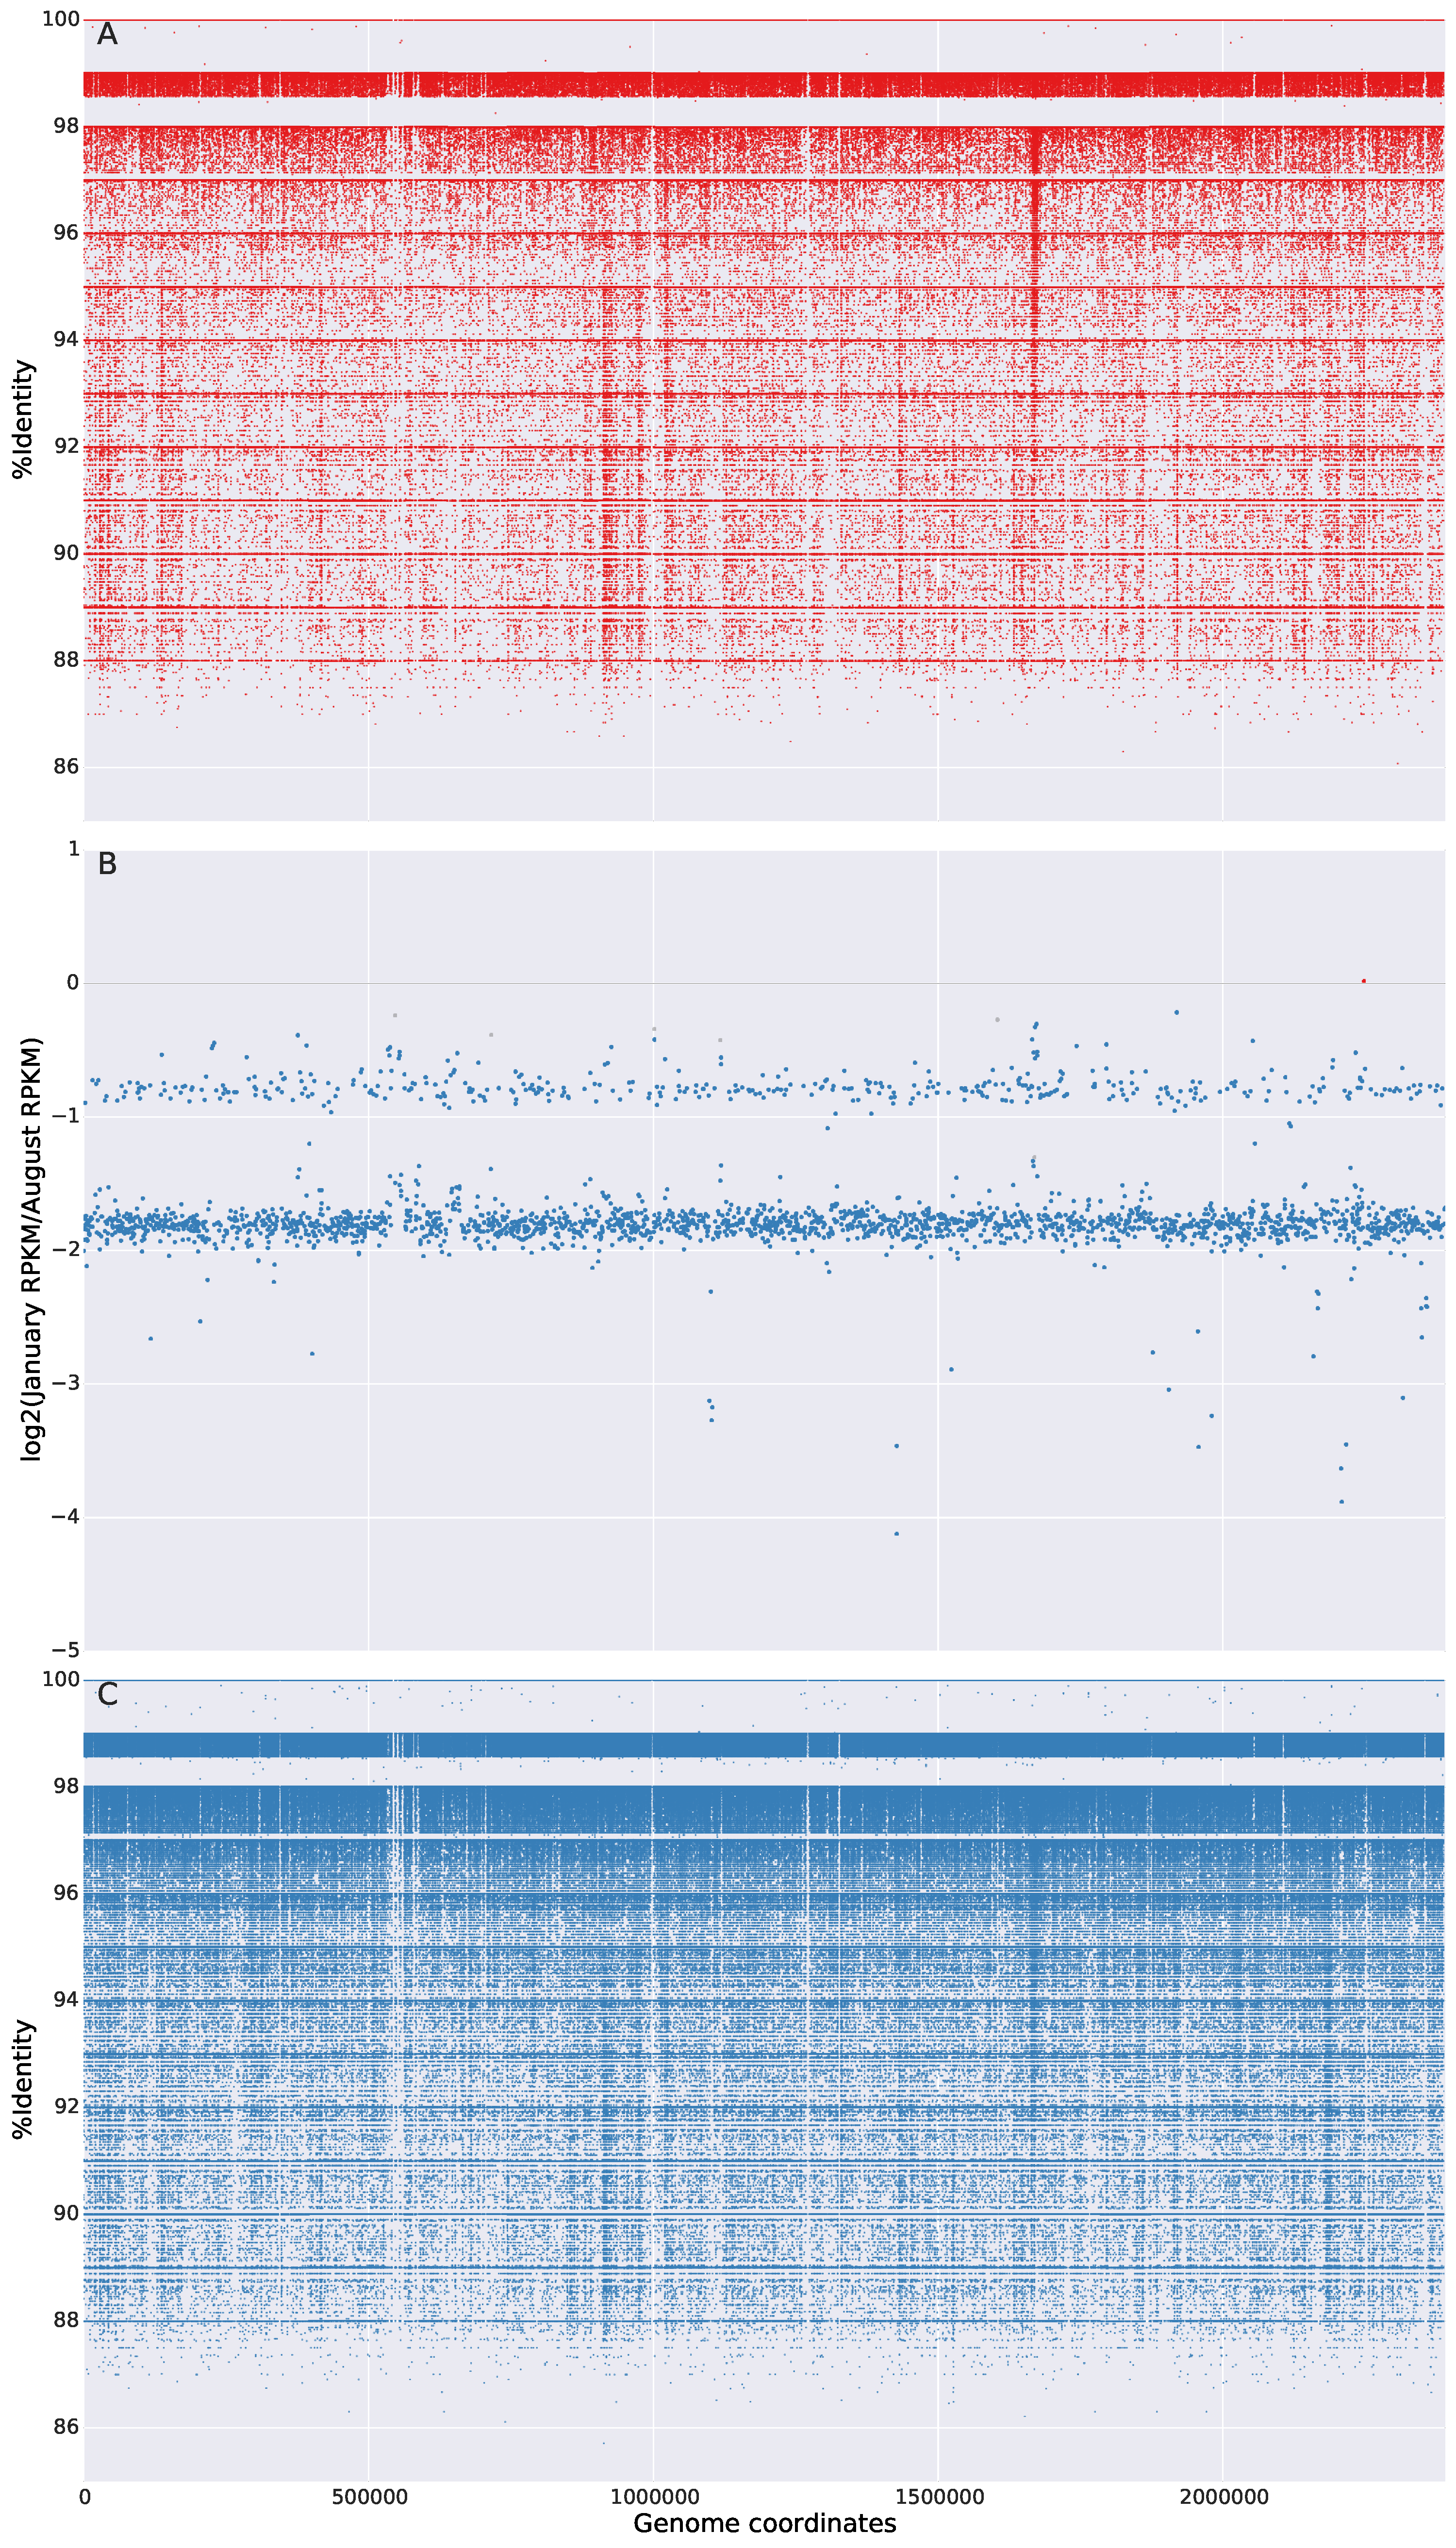
\includegraphics[width=\textwidth,height=0.8\textheight,keepaspectratio]{Chapter5/Figures/coverage_plots/A07HB70_coverage.pdf}
  \caption{Coverage and gene abundance for A07HB70. \textbf{A} and \textbf{C} shows reads recruited to the January and August genomes, respectively. \textbf{B} indicates the number of reads recruited to each individual gene, expressed as RPKM values, where the color indicates the sample from where the read originated (January vs. August.)}
  \label{A07HB70coverage}
\end{figure}

\begin{figure}[!hbtp]
  \centering
  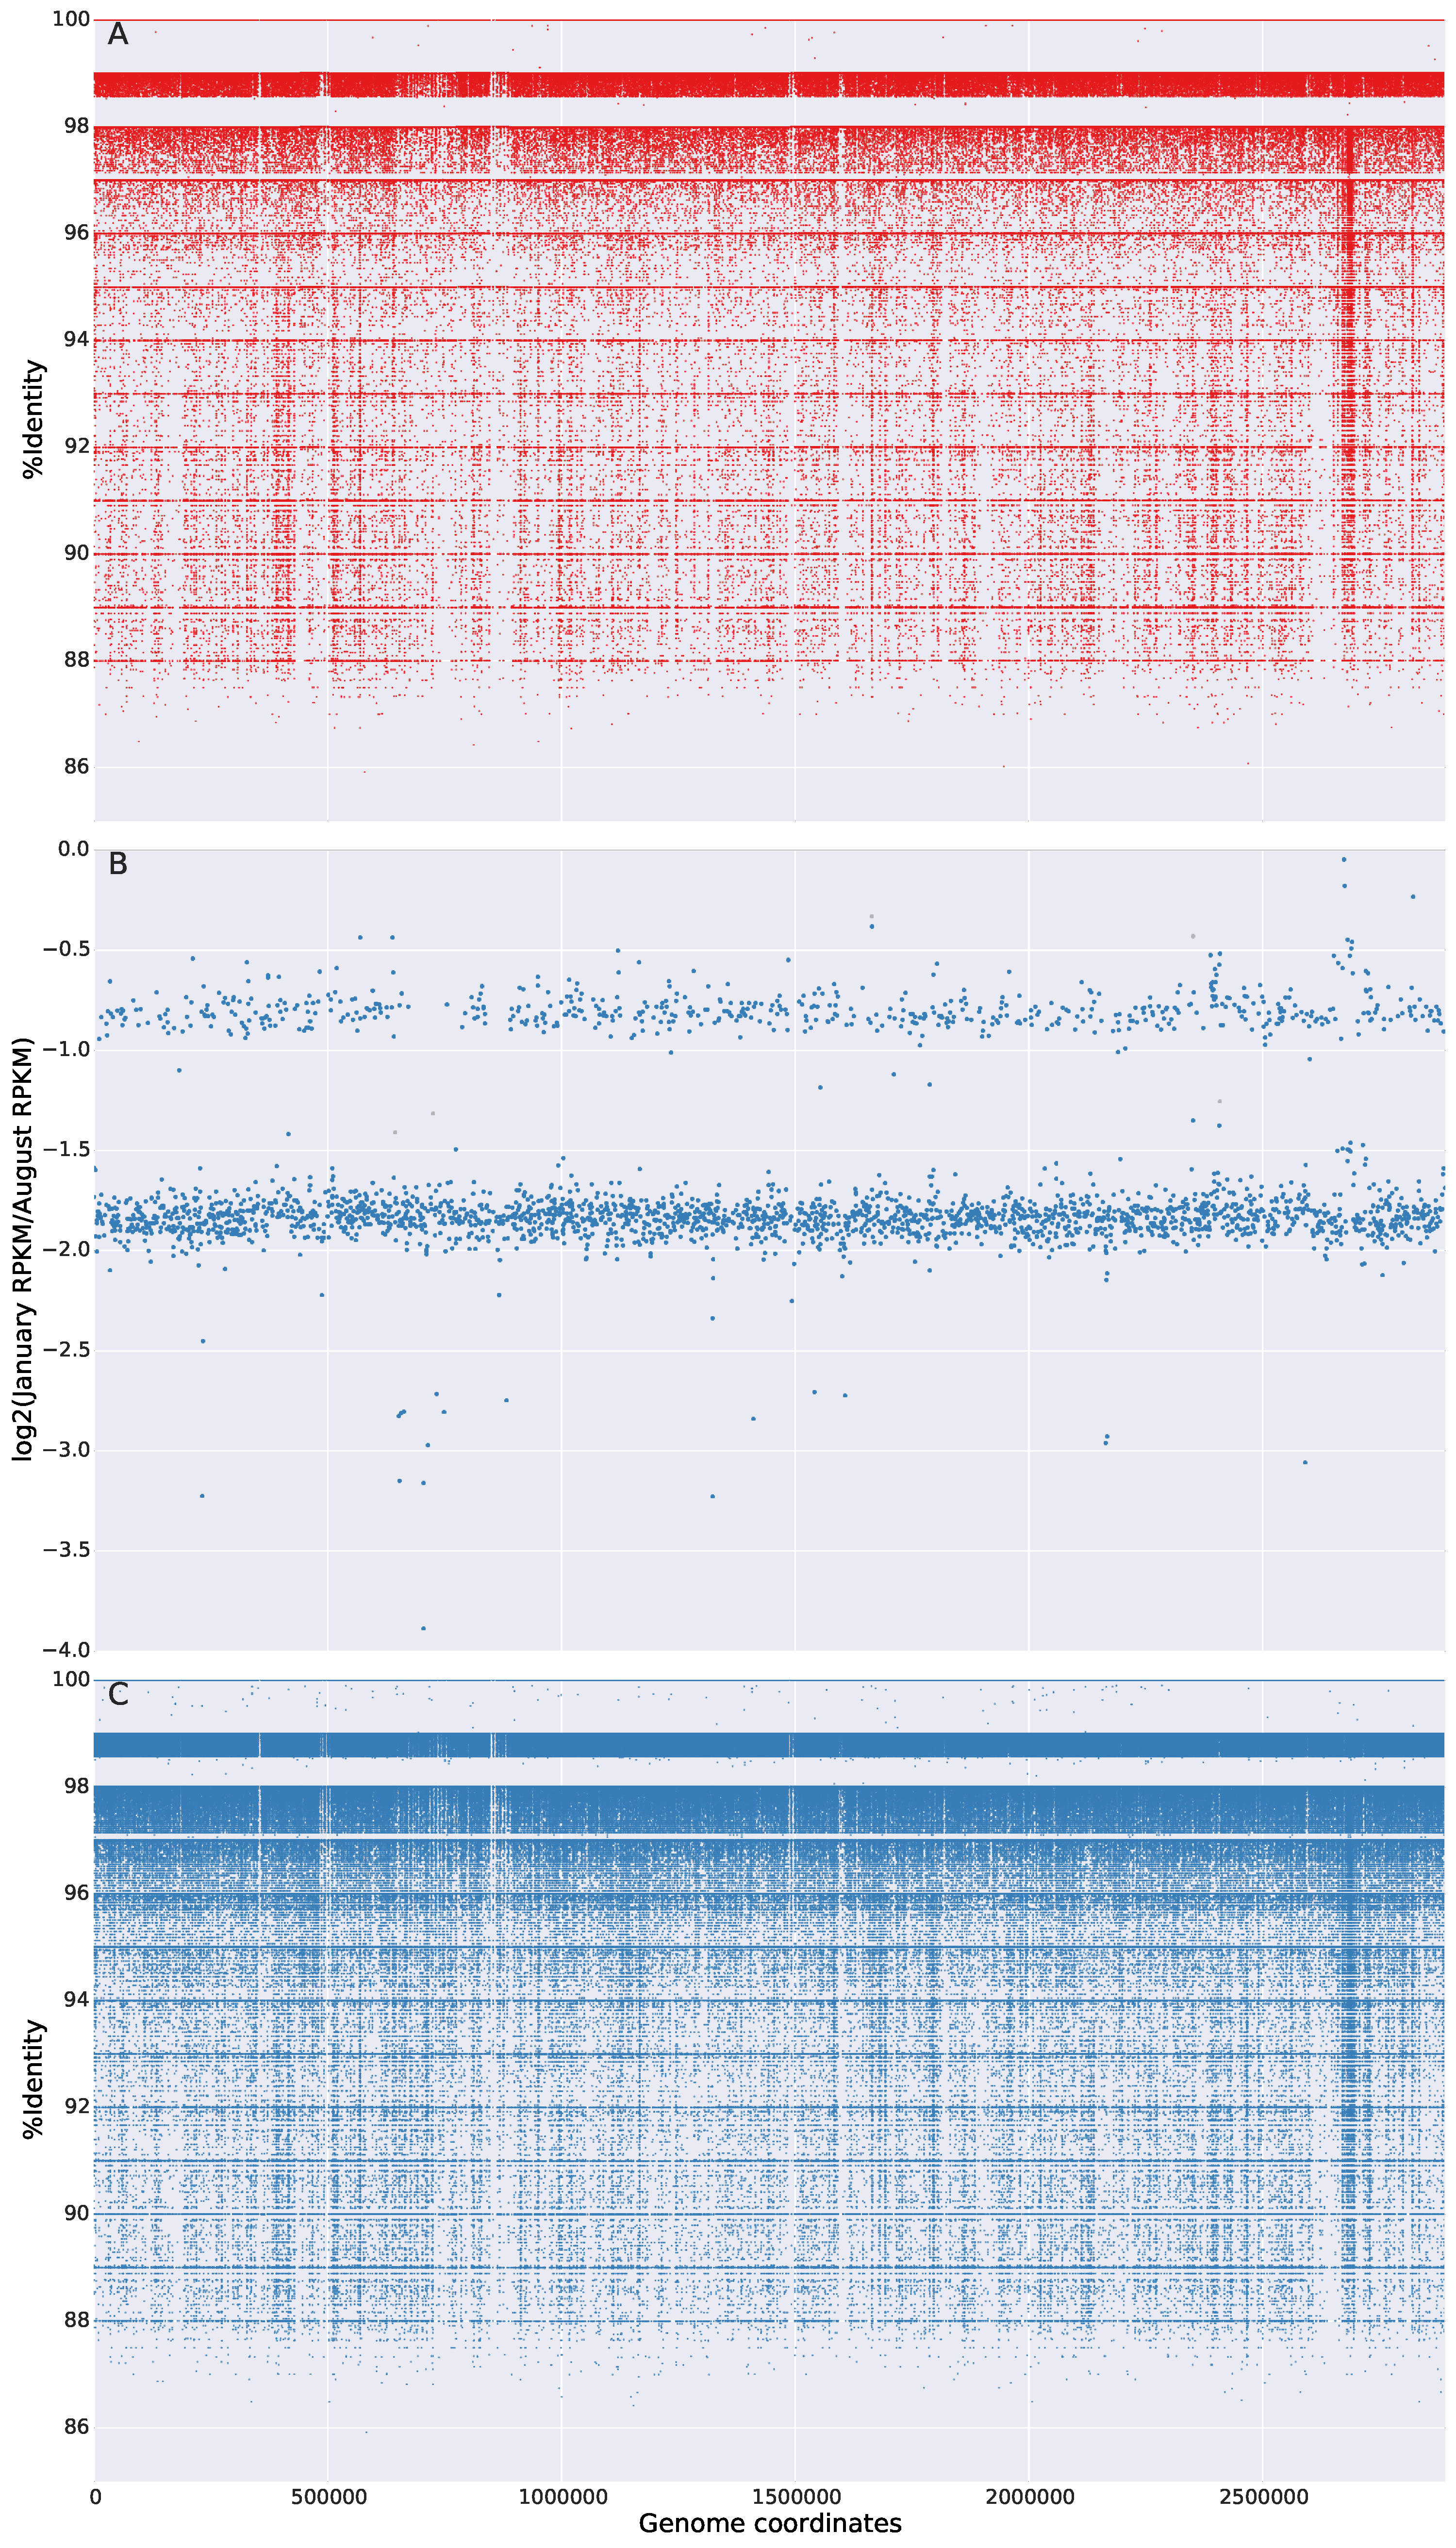
\includegraphics[width=\textwidth,height=0.8\textheight,keepaspectratio]{Chapter5/Figures/coverage_plots/A07HR67_coverage.pdf}
  \caption{Coverage and gene abundance for A07HR67. \textbf{A} and \textbf{C} shows reads recruited to the January and August genomes, respectively. \textbf{B} indicates the number of reads recruited to each individual gene, expressed as RPKM values, where the color indicates the sample from where the read originated (January vs. August.)}
  \label{A07HR67coverage}
\end{figure}

\begin{figure}[!hbtp]
  \centering
  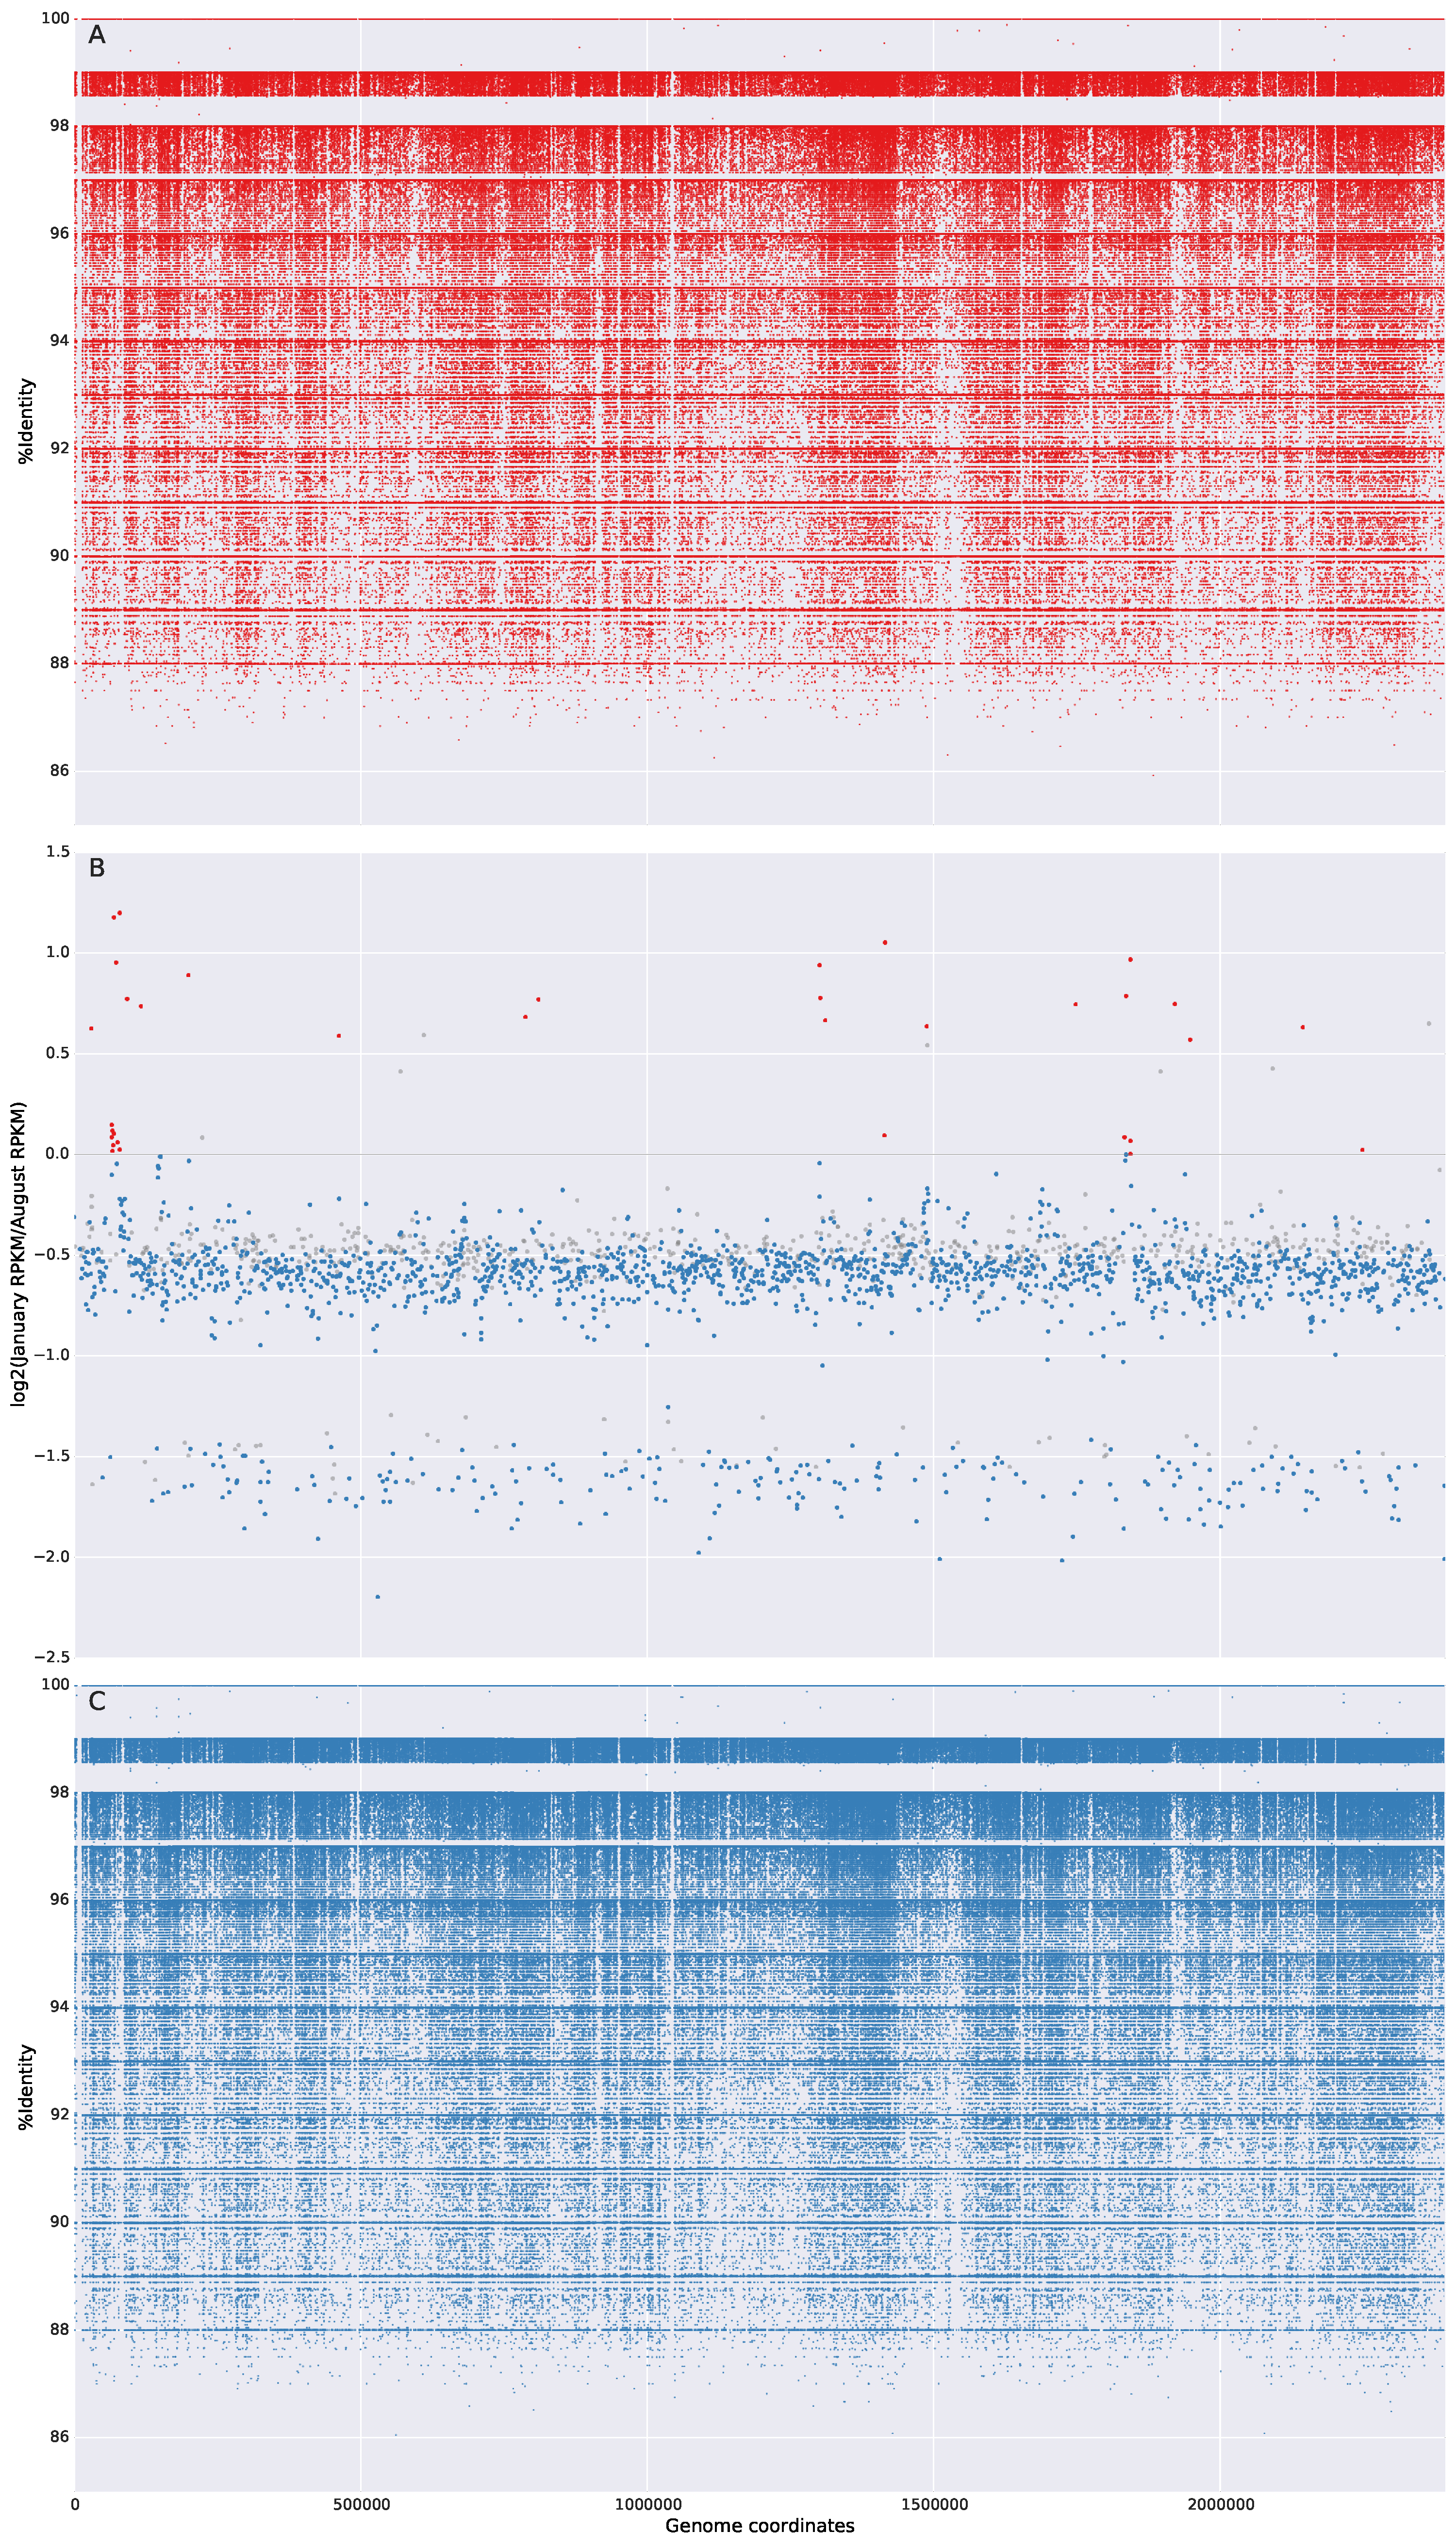
\includegraphics[width=\textwidth,height=0.8\textheight,keepaspectratio]{Chapter5/Figures/coverage_plots/A07HN63_coverage.pdf}
  \caption{Coverage and gene abundance for A07HN63. \textbf{A} and \textbf{C} shows reads recruited to the January and August genomes, respectively. \textbf{B} indicates the number of reads recruited to each individual gene, expressed as RPKM values, where the color indicates the sample from where the read originated (January vs. August.)}
  \label{A07HN63coverage}
\end{figure}

\begin{figure}[!hbtp]
  \centering
  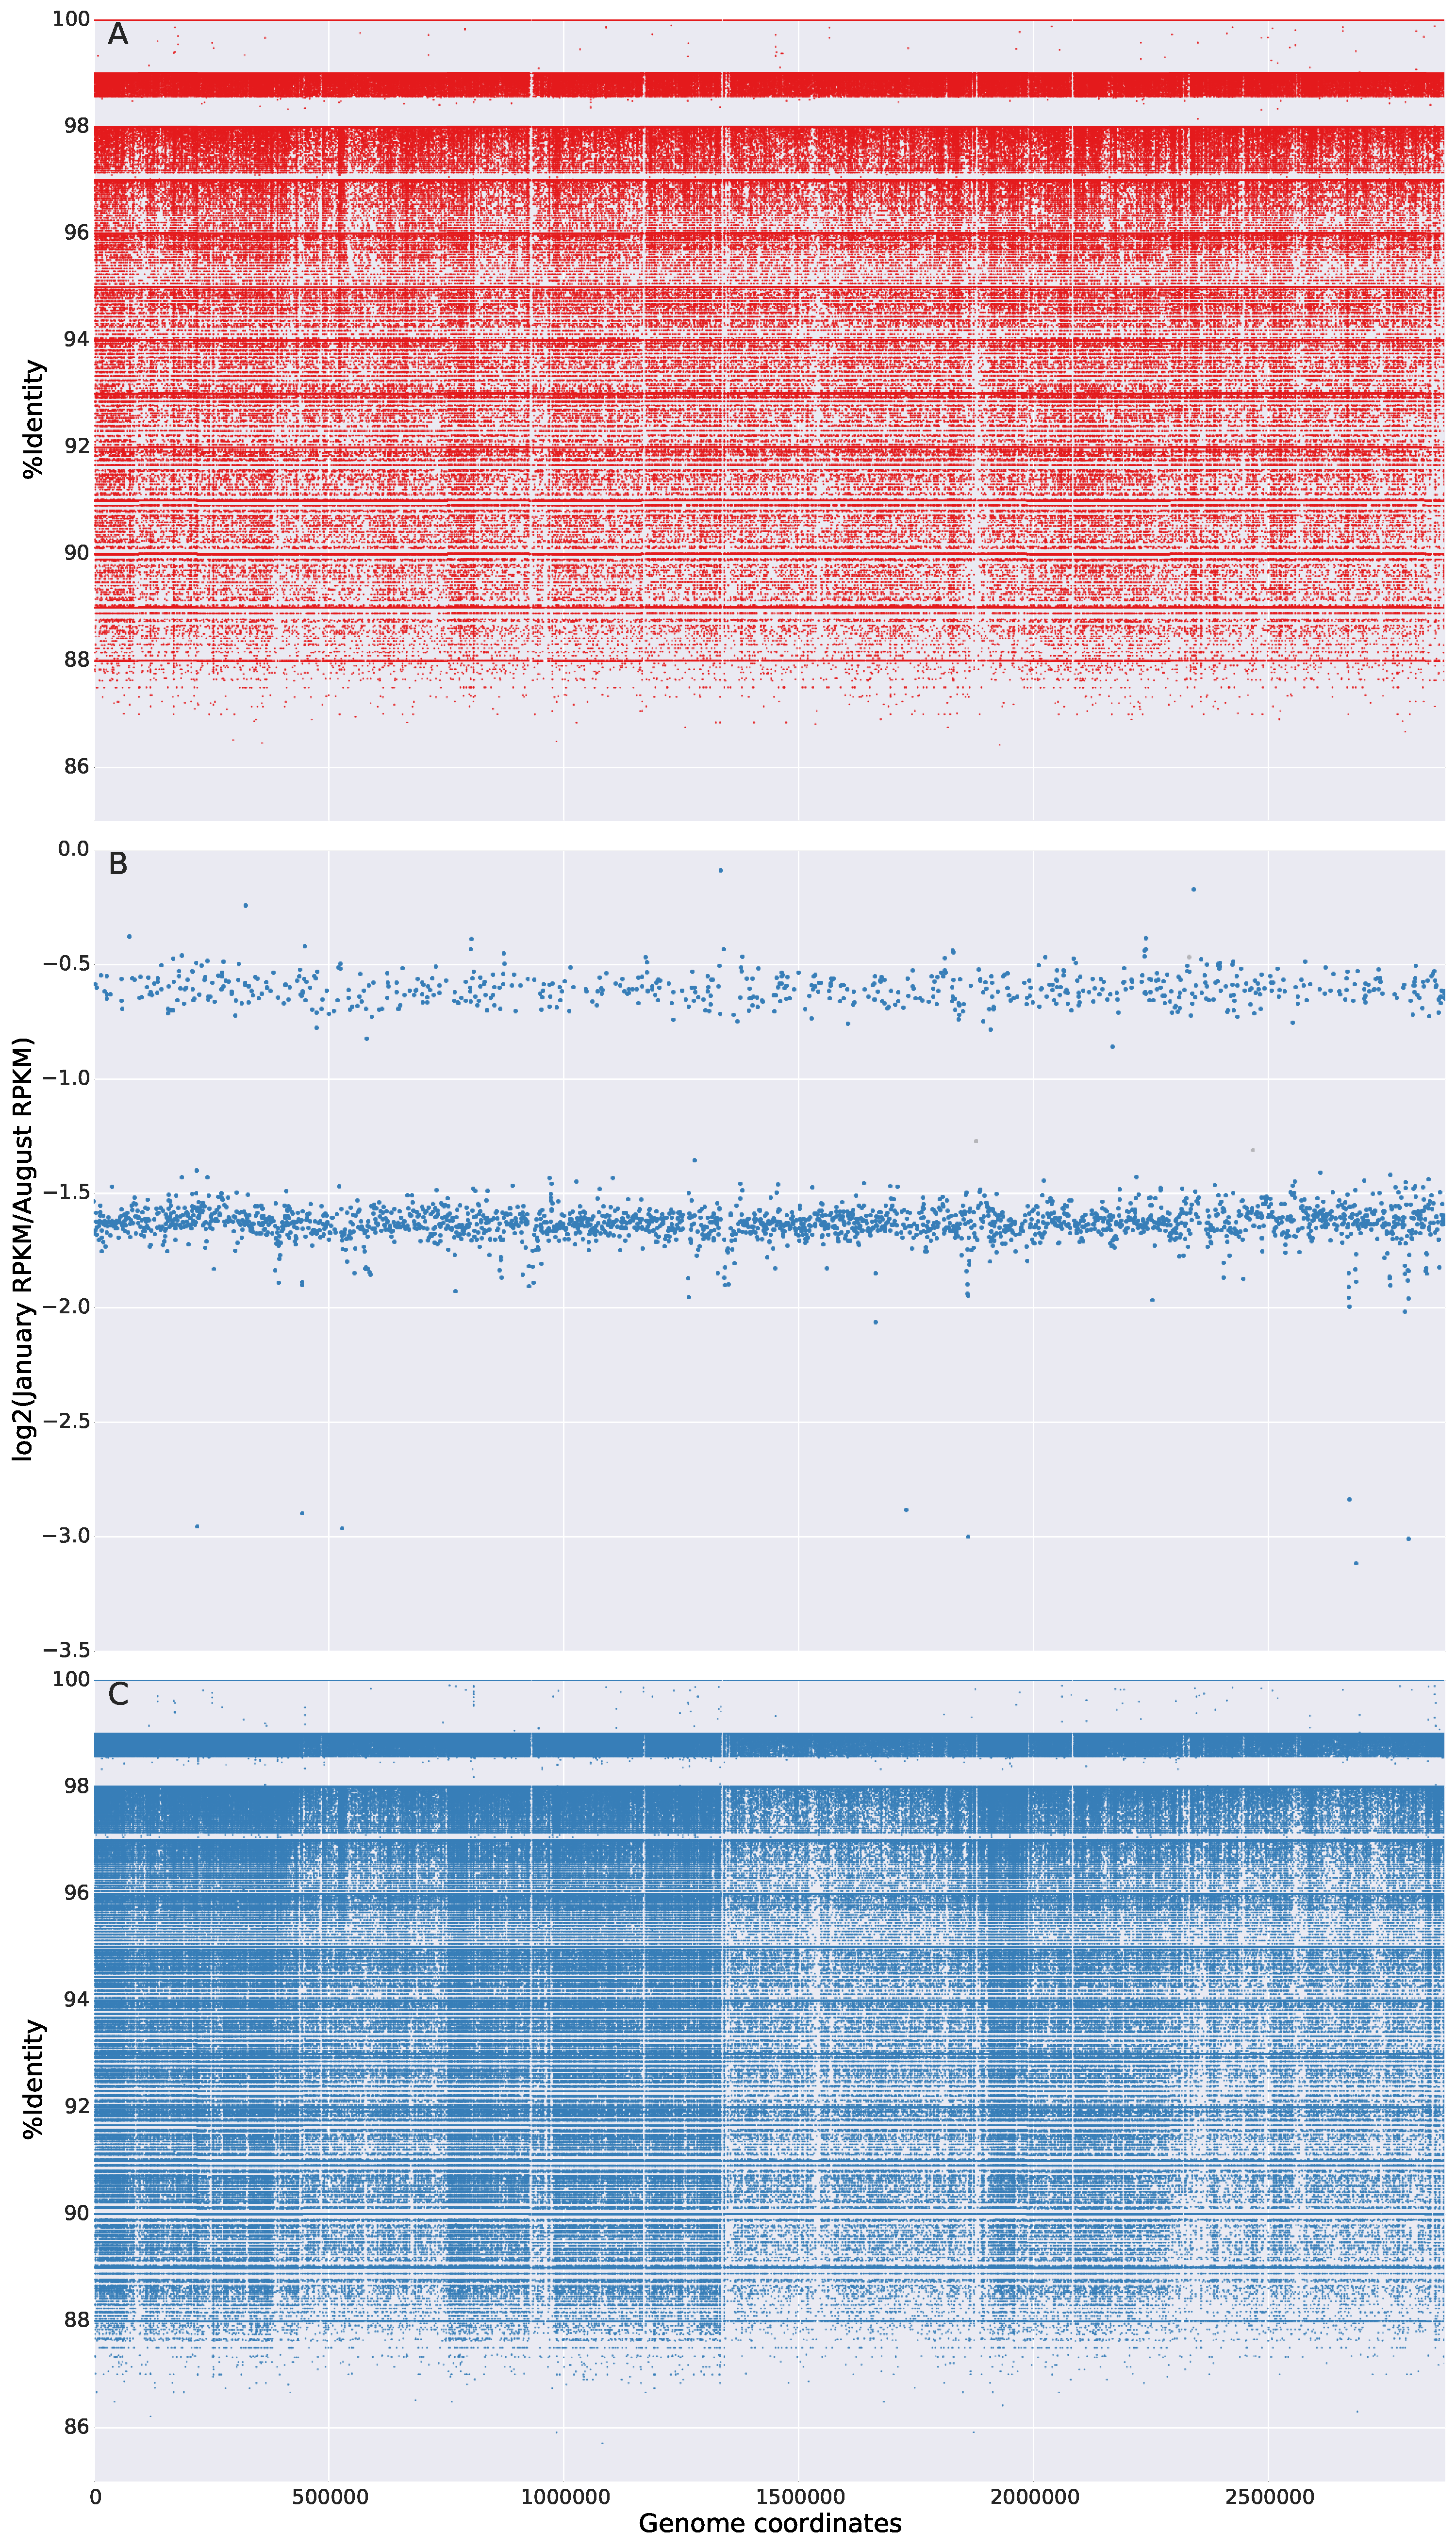
\includegraphics[width=\textwidth,height=0.8\textheight,keepaspectratio]{Chapter5/Figures/coverage_plots/A07HR60_coverage.pdf}
  \caption{Coverage and gene abundance for A07HR60. \textbf{A} and \textbf{C} shows reads recruited to the January and August genomes, respectively. \textbf{B} indicates the number of reads recruited to each individual gene, expressed as RPKM values, where the color indicates the sample from where the read originated (January vs. August.)}
  \label{A07HR60coverage}
\end{figure}

\begin{figure}[!hbtp]
  \centering
  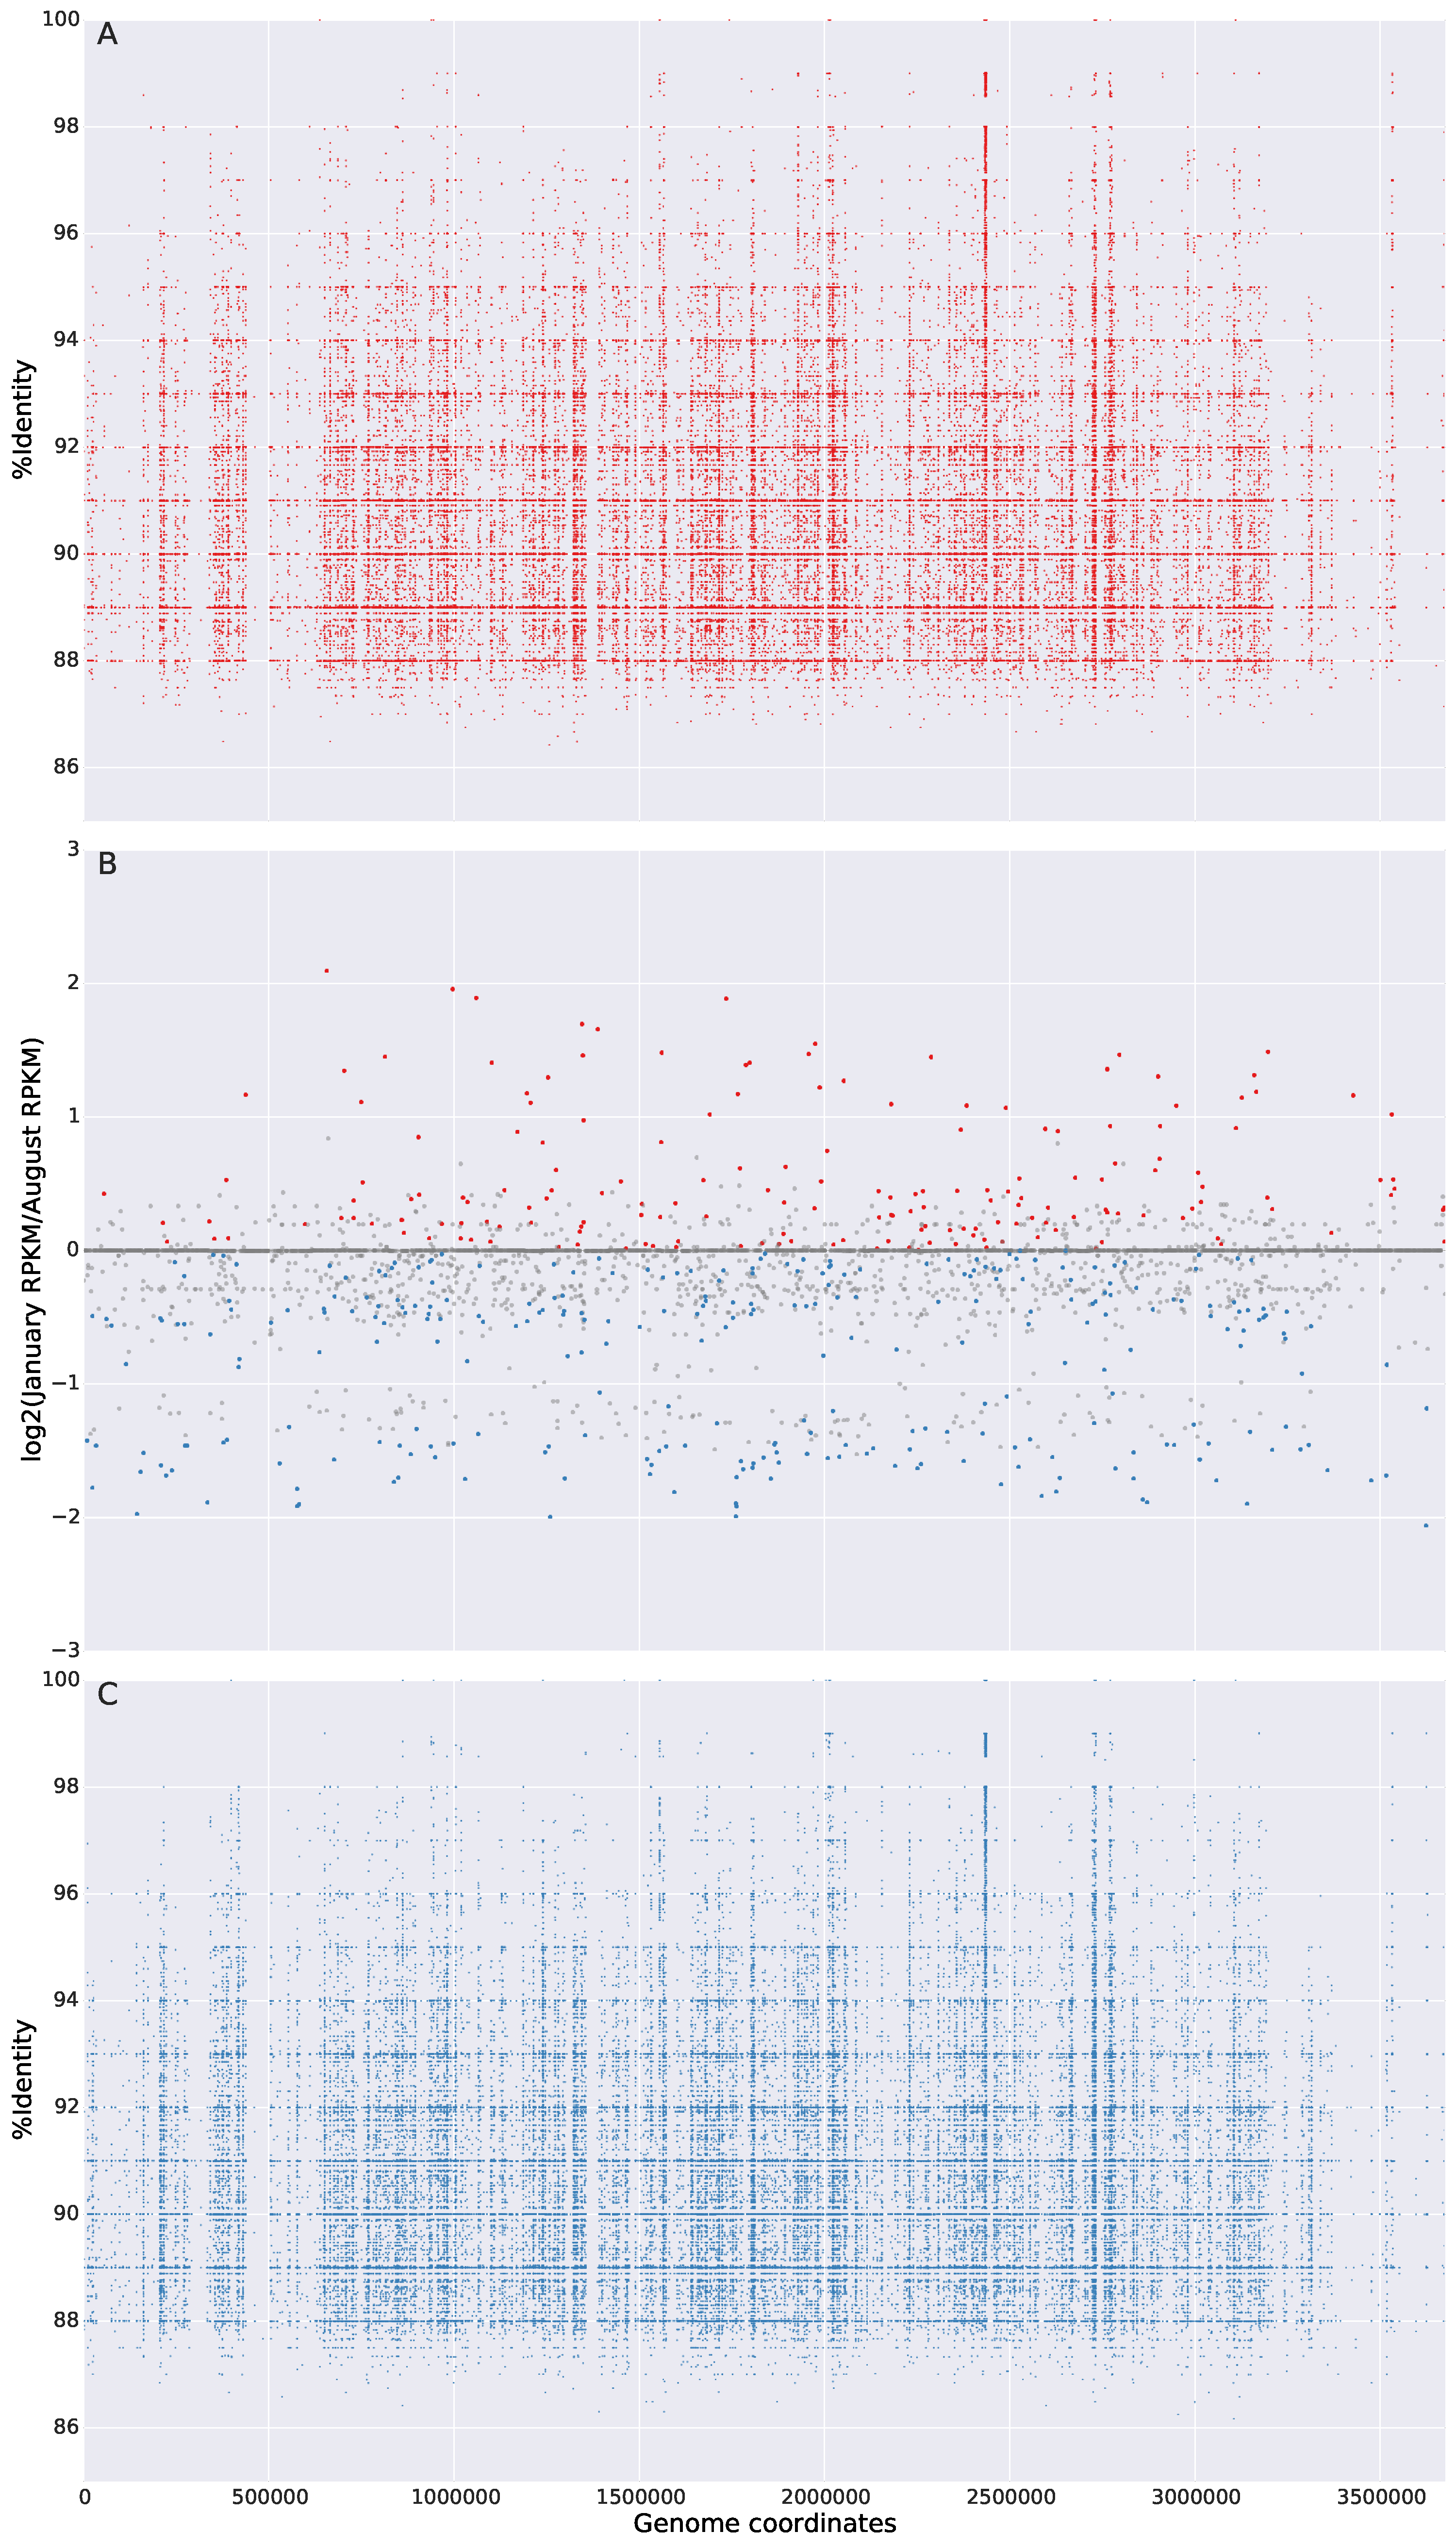
\includegraphics[width=\textwidth,height=0.8\textheight,keepaspectratio]{Chapter5/Figures/coverage_plots/G22_coverage.pdf}
  \caption{Coverage and gene abundance for G22. \textbf{A} and \textbf{C} shows reads recruited to the January and August genomes, respectively. \textbf{B} indicates the number of reads recruited to each individual gene, expressed as RPKM values, where the color indicates the sample from where the read originated (January vs. August.)}
  \label{G22coverage}
\end{figure}

\begin{figure}[!hbtp]
  \centering
  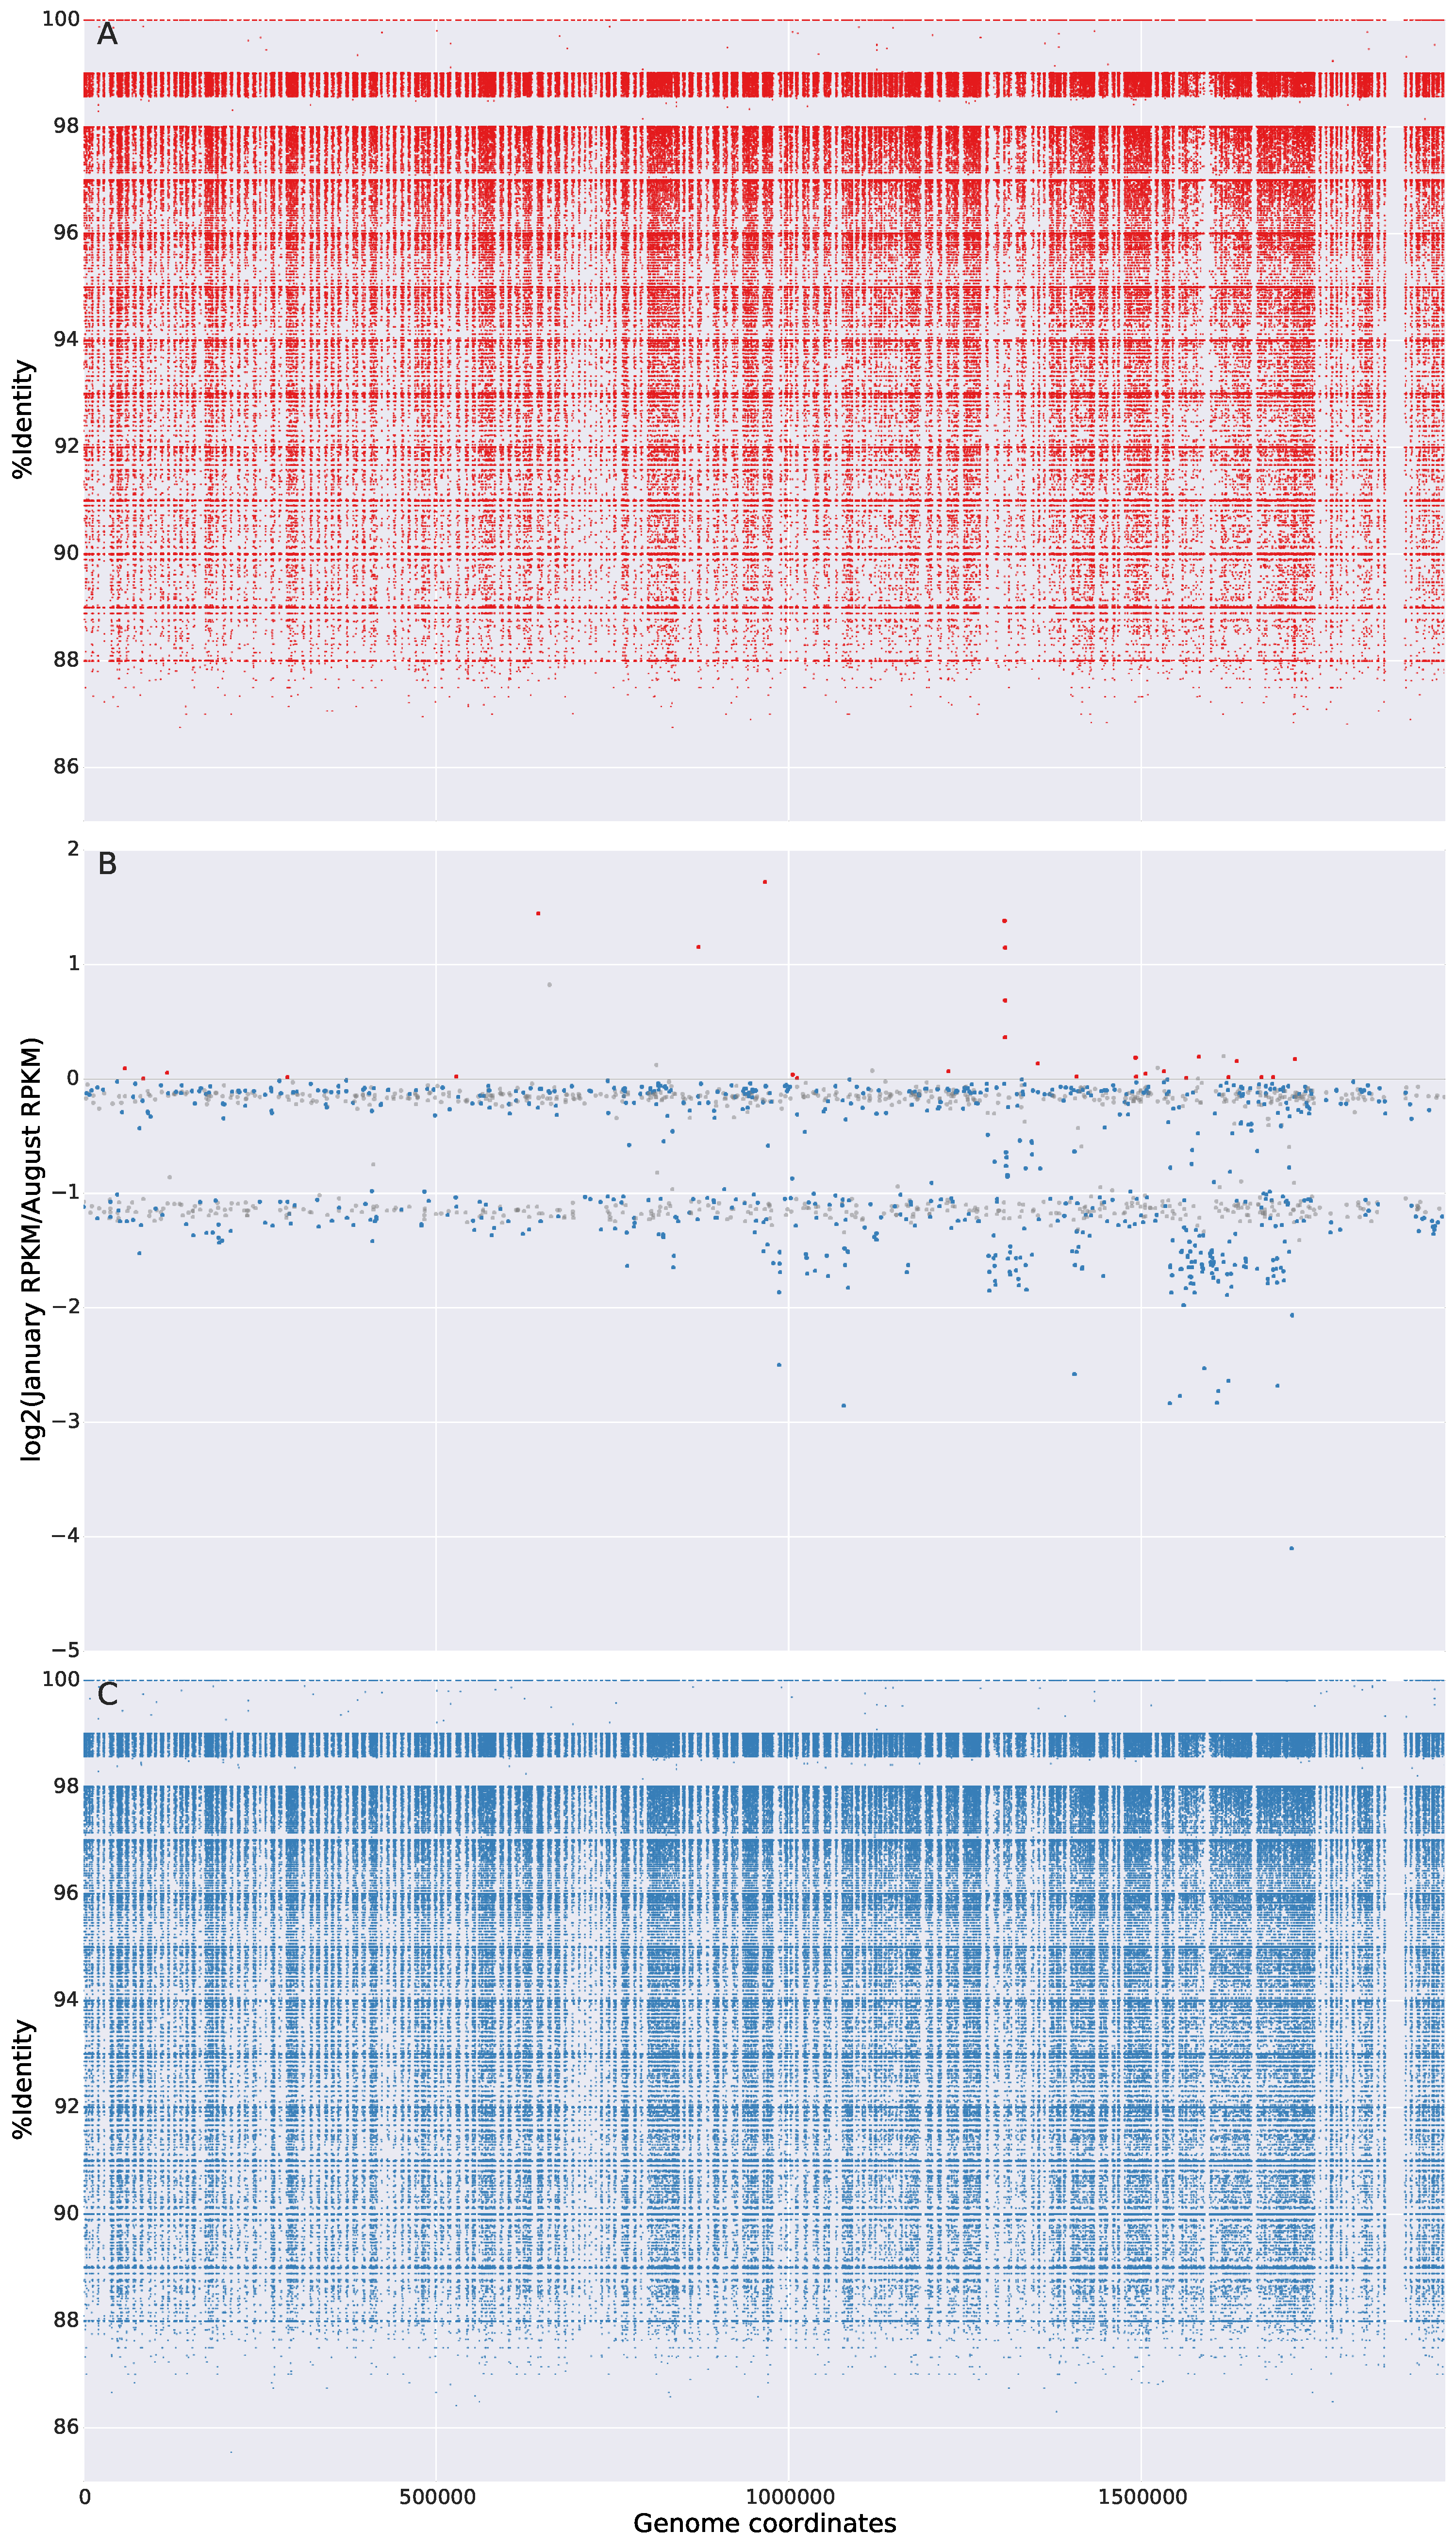
\includegraphics[width=\textwidth,height=0.8\textheight,keepaspectratio]{Chapter5/Figures/coverage_plots/J07SB_coverage.pdf}
  \caption{Coverage and gene abundance for J07SB. \textbf{A} and \textbf{C} shows reads recruited to the January and August genomes, respectively. \textbf{B} indicates the number of reads recruited to each individual gene, expressed as RPKM values, where the color indicates the sample from where the read originated (January vs. August.)}
  \label{J07SBcoverage}
\end{figure}
